\documentclass[english]{upeeei}
\usepackage[latin9]{inputenc}
\setcounter{secnumdepth}{3}
\setcounter{tocdepth}{3}
\usepackage[active]{srcltx}
\usepackage{float}
\usepackage{units}
\usepackage{graphicx}
\usepackage{url}
\usepackage{pgfgantt}
\usepackage{amsmath}

\makeatletter

\providecommand{\LyX}{L\kern-.1667em\lower.25em\hbox{Y}\kern-.125emX\@}
\providecommand{\tabularnewline}{\\}

\@ifundefined{showcaptionsetup}{}{%
 \PassOptionsToPackage{caption=false}{subfig}}
\usepackage{subfig}
\makeatother

\usepackage{babel}
\begin{document}

\title{Development of a 3D-Printed Quadrupedal Robot with Distributed Joint Control} 

\author{
Jiego Benjamin Osea Guanzon\\ 2015-07906\\ \emph{B.S. Electronics and Communications Engineering}
\and
}

%%
%% Month and year of submission/graduation
\degreeyear{2019} 
\degreesemester{December} 

% Put your advisers here:
\chair{Nicolette Ann Arriola MSEE} 
\othermembers{~}
\numberofmembers{2} 

\field{Electrical/Computer/Electronics and Communications Engineering} 
\campus{Diliman} 

\maketitle 
% \approvalpage 
% \copyrightpage 
\begin{abstract} 

In a \emph{single} well-written paragraph, this is what we'd like to do.  Try to cover Need, Solution, Differentiation, Benefit (NSDB).  Use the content of this template as an example for formatting your proposal document, \textbf{NOT} as a strict guide for the flow of your discussion and what your proposal must contain.

\abstractsignature\end{abstract}

\begin{frontmatter} 

\setlength{\parskip}{0pt}

\tableofcontents{}

\listoffigures

\listoftables

\end{frontmatter} 

\def\MASTERDOC{true}

\cleardoublepage{}

\chapter{Introduction\label{cha:Introduction}}

\section{Background of the Project}

Legged robots have several advantages over other types of mobile robots. While wheeled robots can move at high speeds, their operation is limited to relatively flat environments. Legged robots, on the other hand, have higher degrees of freedom (DOF) allowing them to operate in uneven and unpredictable terrain. Discrete motion trajectories and multiple limbs translate to higher maneuverability and flexibility coupled with stability and fault tolerance \cite{quadrobotlegs}.

However, bipedal (two-legged) robots have periods of instability during locomotion where only one leg is in contact with the ground. Other configurations with three or more legs have the characteristic of being stable as long as their center of mass is within the support polygon defined by the position of their legs. While having more legs usually means higher stability, it has the drawback of requiring more actuators and having more complex gaits. Quadrupedal robots, or four-legged robots, offer a robust middle-ground platform that has better load capacity and higher stability than bipedal robots while using fewer actuators compared to higher leg-count robots \cite{quadrobotlegs}.

Quadrupedal robots, such as Boston Dynamic's Bigdog \cite{bigdog} and MIT's Cheetah 3 \cite{mitcheetah3}, are generally inaccessible to most researchers due to their high cost and large size. Recent developments for the Cheetah 3 robot include MIT's state-of-the-art Mini Cheetah \cite{minicheetah}. It has a smaller form-factor, approximately 60\% of the Cheetah 3, and costs approximately \$3600. While the cost is significantly smaller that its predecessor, it is still too expensive for most experimental and research purposes.

\section{Project Objectives}

The project aims to develop a prototype of a cost-efficient 12-DOF quadrupedal robot. Proprioceptive actuators, with off-the-shelf brushless DC (BLDC) motors, are used to drive the joints to allow locomotion in uneven terrain. Custom joint controllers are to be used with the proprioceptive actuators, while a custom main controller is to be used to handle the entire robot.

The project also aims to create a robust platform that is to be used with gait experimentation and other quadrupedal robot research.

\section{Project Overview}

The project can be divided into two major parts: design and control. The block diagram of the project is shown in Figure \ref{fig:project-block-diagram}.

\begin{figure}[H]
\begin{centering}
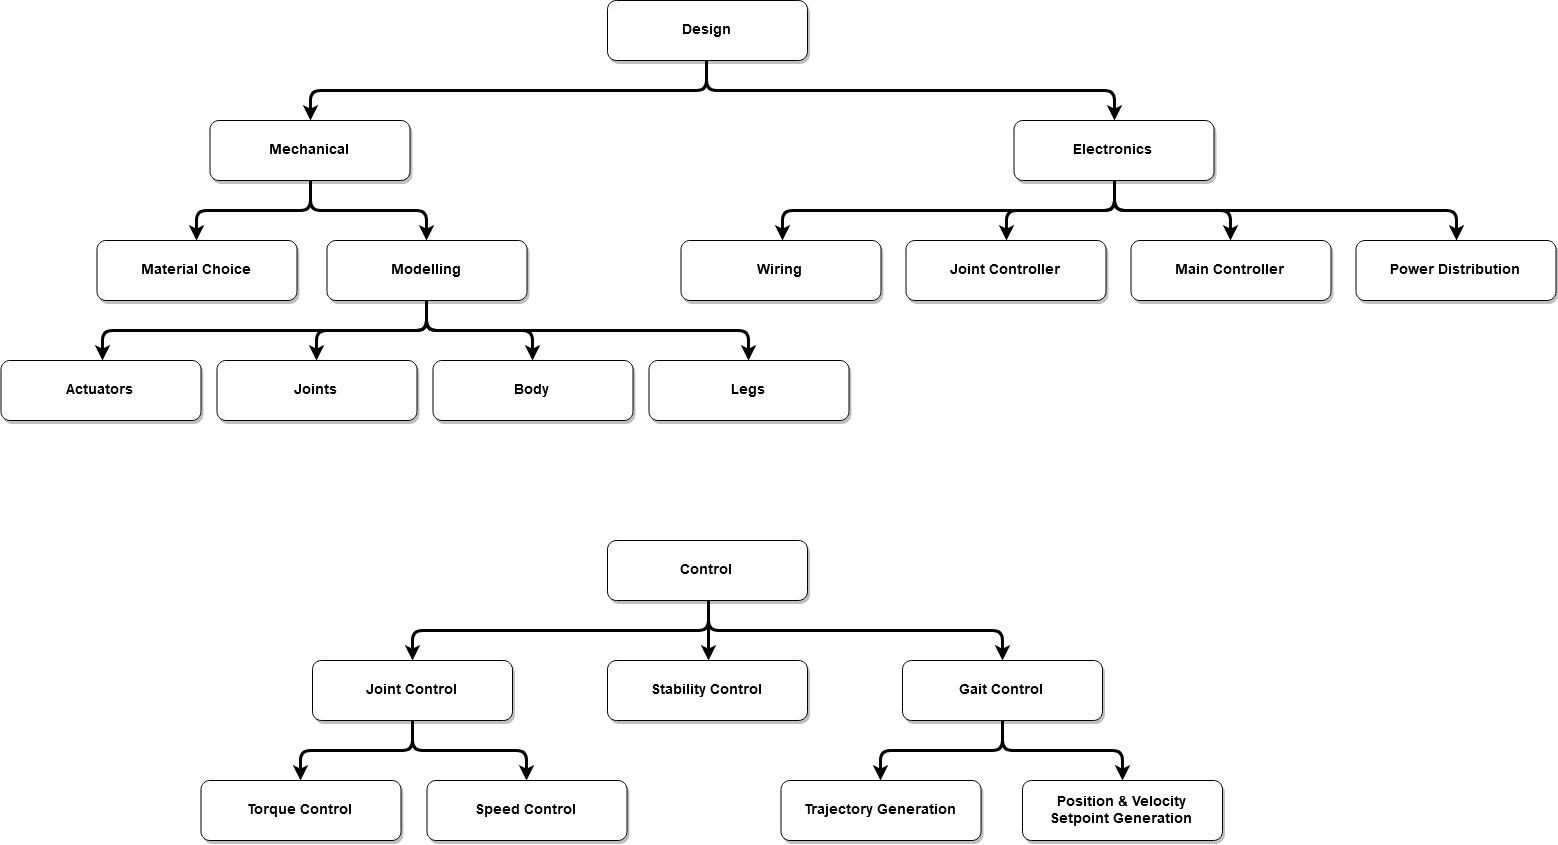
\includegraphics[width=1.0\columnwidth]{images/project_block_diagram}
\par\end{centering}
\caption{Project Block Diagram\label{fig:project-block-diagram}}
\end{figure}

\subsection{Design}

The design part of the project can be further divided into two parts: mechanical and electronics design. 

Mechanical design of the quadrupedal robot involves the modelling and construction of the actuator, joints, legs, and body of the robot. Modelling is done and simulated using Fusion360. Fused Deposition Modelling (FDM) 3D-printing is used to fabricate each part with polylactic acid (PLA). The actuator is comprised of a BLDC motor coupled to a 3D-printed planetary gearbox with a 6.125 reduction ratio. The joints are driven either directly by the actuator or by a timing belt.

Electronics design of the quadrupedal robot involves the design and fabrication of custom main and joint controllers. Both controllers utilize a dsPIC33 microcontroller while the joint controller has a smart gate driver integrated circuit (IC) which drives a three-phase power inverter. The method of power delivery to each actuator is also considered in this design phase. The block diagram of both controllers are shown in Figure \ref{fig:controller-diagrams}

\begin{figure}[H]
\begin{centering}
\subfloat[Joint Controller Topology]{\begin{centering}
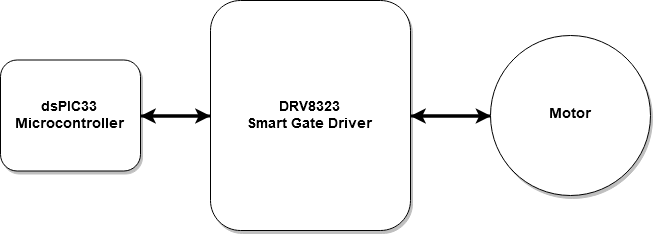
\includegraphics[width=0.45\columnwidth]{images/joint_controller}
\par\end{centering}
}
\par\end{centering}
\begin{centering}
\subfloat[Main Controller Topology]{\begin{centering}
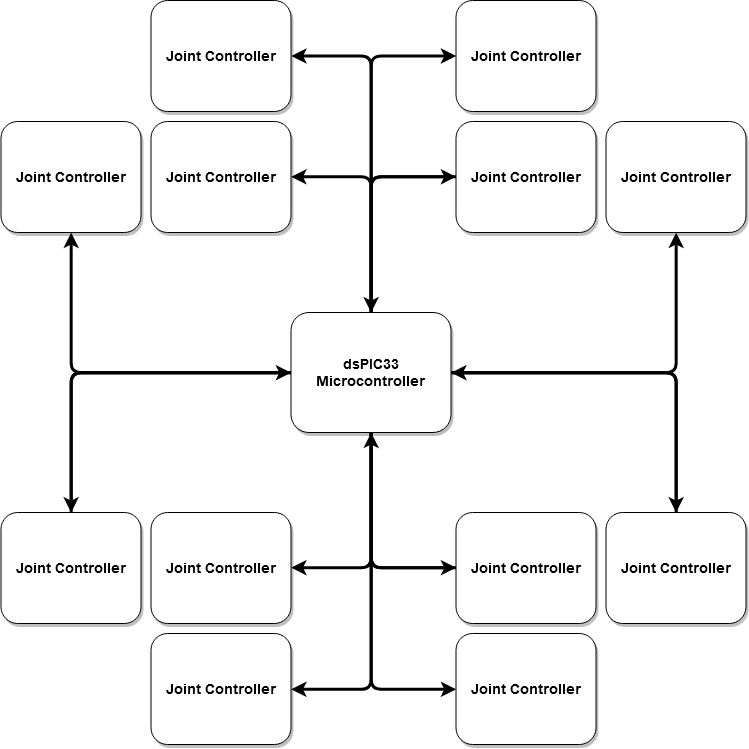
\includegraphics[width=0.6\columnwidth]{images/main_controller}
\par\end{centering}
}
\par\end{centering}
\caption{Controller Topologies\label{fig:controller-diagrams}}
\end{figure}

\subsection{Control}

The control part of the project can be further divided into three parts: joint, stability, and gait control.

Joint control, which is local to each motor controller, is responsible for the low level control of output torque and speed of each actuator. Stability control is responsible for the overall balance of the robot. Gait control is responsible for generating the trajectories of each leg and sending positional and velocity data setpoints to each actuator. Both stability and gait control are processed by the main microcontroller of the quadruped.

\section{Documentation Flow and Organization}

Chapter 2 starts with the discussion of different types of actuators and mechanical legs used for legged robots. Then, the mechanical properties of thermoplastic materials commonly used in 3D printing are compared with one another. Control theory of quadrupedal robots are touched upon at the end of the chapter.

Chapter 3 states the project's main objectives and discusses the problems it aims to solve.

\cleardoublepage{}

\chapter{Related Work\label{cha:RRW}}

\section{Actuators}

Actuators are considered as the driving force behind each joint of a robot. These are essential to any robot since without these, motion and operation will not be possible. Their design and architecture determines the efficiency of the robot and the type of control to be used. Three main types of actuators used in legged robotics that are to be discussed in this section are: hydraulic, series-elastic, and proprioceptive actuators.

Hydraulic actuators utilize different types of fluids to drive the robot's joints. They usually have high force density with high impact robustness, where the load from impacts are distributed evenly over a large surface area in the hydraulic channels. The use of hydraulic actuators typically do not add significant amounts of mass and inertia to the limbs, which is ideal for high-speed legged locomotion \cite{minicheetah}. However, hydraulic actuators have their drawbacks, such as having highly non-linear dynamic behaviors. This makes their closed-loop control extremely complicated. They are also ineffecient, compared to electric actuators, due to energy leakage concerning the hydraulic fluid \cite{controlhydraulic}.

Boston Dynamics' Bigdog, one of the most popular and well-known quadrupedal robot, utilizes a two-stroke internal combustion engine to drive its hydraulic actuators \cite{bigdog}. The actuators are low-friction hydraulic cylinders with two-stage servovalves. An on-board heat-exchanger is required to cool the the hydraulic oil used and the combustion engine. These add weight to the robot with its overall weight totalling to 109 kg. The robot topology is shown in Figure \ref{fig:bigdog}.

\begin{figure}[H]
\begin{centering}
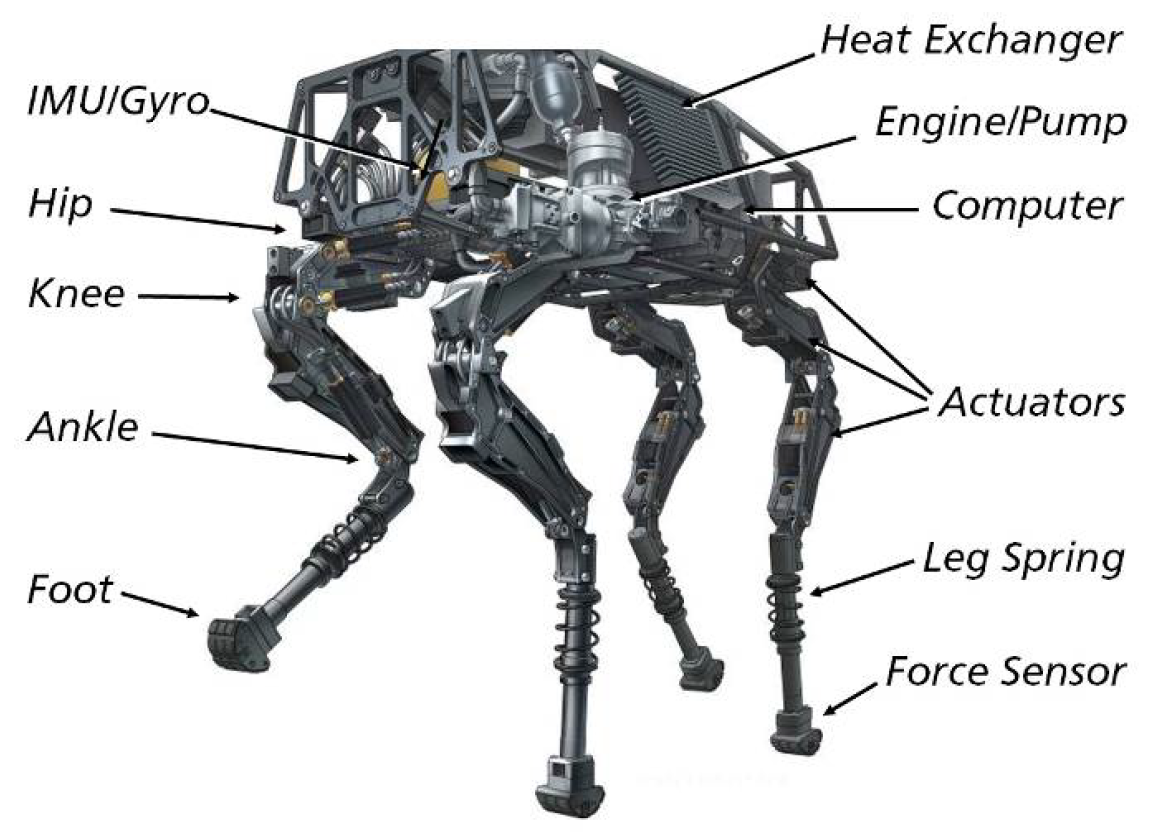
\includegraphics[width=0.5\columnwidth]{images/bigdog}
\par\end{centering}
\caption{Bigdog Robot Topology\label{fig:bigdog}}
\end{figure}

The second type of actuator to be discussed is the series-elastic actuator (SEA). This type of actuator typically uses a high-geared electric motor and adds an elastic spring in series between the output and the load. The block diagram of a SEA is shown in Figure \ref{fig:sea-block-diagram} \cite{sea}.

\begin{figure}[H]
\begin{centering}
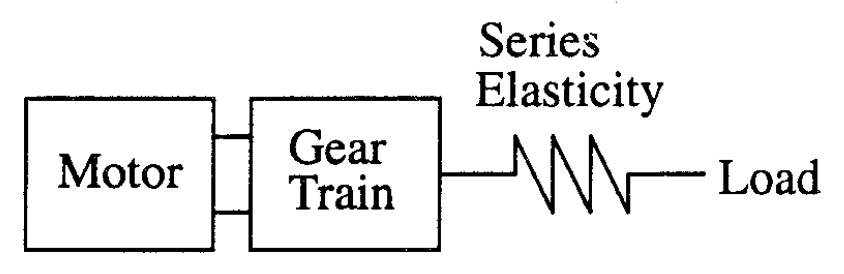
\includegraphics[width=0.5\columnwidth]{images/sea_block_diagram}
\par\end{centering}
\caption{Series-elastic Actuator Block Diagram\label{fig:sea-block-diagram}}
\end{figure}

The addition of a series elastic spring essentially filters the high-frequency impact forces on the actuator, causing less peak force on the gears. This, however, also filters the high-frequency output of the actuator, creating a trade-off between impact tolerance and small motion bandwidth. Series-elasting actuators can also be used as a form of energy storage. This energy storage can be highly beneficial to legged locomotion because it increases its energy efficiency \cite{sea}. Force control problems with SEAs are turned into position control problems where the output force is directly proportional to the positional difference of the series elastic spring muliplied by its spring constant. Therefore, series-elastic actuators require more positional sensors in order to compute and control force output. This adds mechanical complexity and cost to the actuator \cite{minicheetah}.

The ANYmal quadrupedal robot uses highly-integrated modular series-elastic actuators, which are called ANYdrive. It uses high-torque motors coupled to harmonic drive gears which are in series with a rotational spring. Joint position and spring deflection are measured using absolute positional sensors that have a positional and torque accuracy of 0.025\textdegree and 0.08 Nm, respectively \cite{anymal2}. The ANYdrive actuator is shown in Figure \ref{fig:anydrive} \cite{anymal2}.

\begin{figure}[H]
\begin{centering}
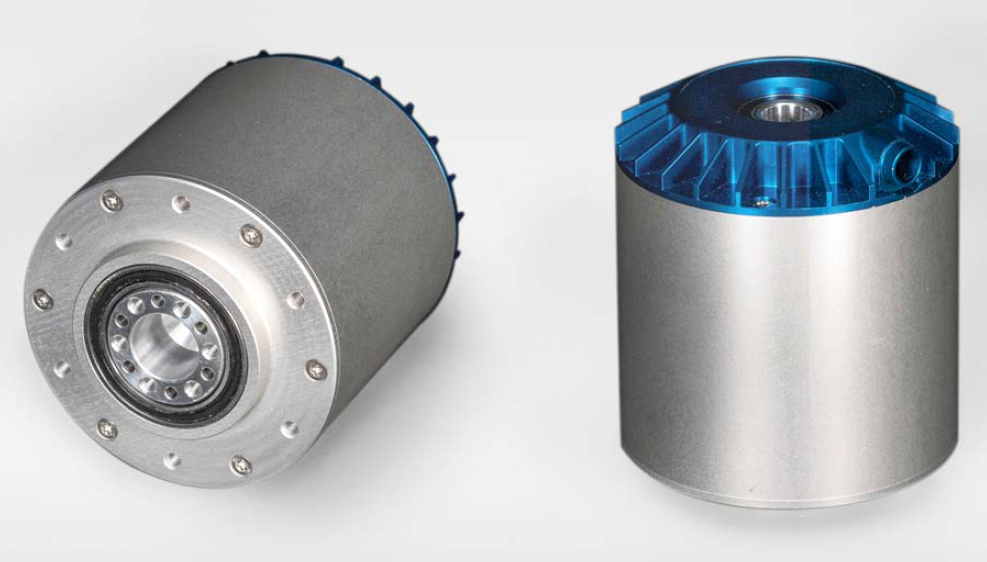
\includegraphics[width=0.4\columnwidth]{images/anydrive}
\par\end{centering}
\caption{ANYdrive Series-Elastic Actuator\label{fig:anydrive}}
\end{figure}

The third and last type of actuator to be discussed is the proprioceptive actuator. This type of actuator uses high torque density electric motors coupled to a transmission stage with a low gear reduction ratio to achieve high torque bandwidth torque control and high backdrivability \cite{minicheetah, cheetah3actuator}. This actuator type increases mechanical simplicity and reduces part count as it eliminates the need for series-elastic springs and requires only one position sensor for the motor rotor. The topology of proprioceptive actuators is shown in Figure \ref{fig:proprioceptive-actuator} \cite{cheetah3actuator}.

\begin{figure}[H]
\begin{centering}
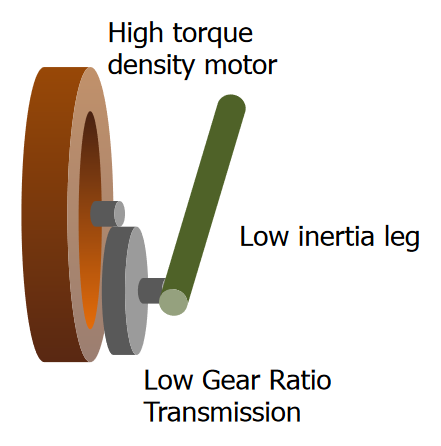
\includegraphics[width=0.3\columnwidth]{images/proprioceptive}
\par\end{centering}
\caption{Proprioceptive Actuator Topology\label{fig:proprioceptive-actuator}}
\end{figure}

MIT's Cheetah 3 and Mini Cheetah uses custom proprioceptive actuators to drive their robot's joints. The Cheetah 3 uses custom high torque density BLDC motors coupled to a single-stage planetary gear train with a 7.67 gear reduction ratio \cite{mitcheetah3}. The Mini Cheetah, on the other hand, uses a modified off-the-shelf brushless motor with the output plate coupled to a planetary gearbox with a 6 gear reduction ratio. These are attached to a custom-made slim-profile aluminum housing along with its motor controller and position sensor. The Mini Cheetah actuator is shown in Figures \ref{fig:mini-cheetah-actuator} \cite{minicheetah}.

\begin{figure}[H]
\begin{centering}
\subfloat[Mini Cheetah Actuator]{\begin{centering}
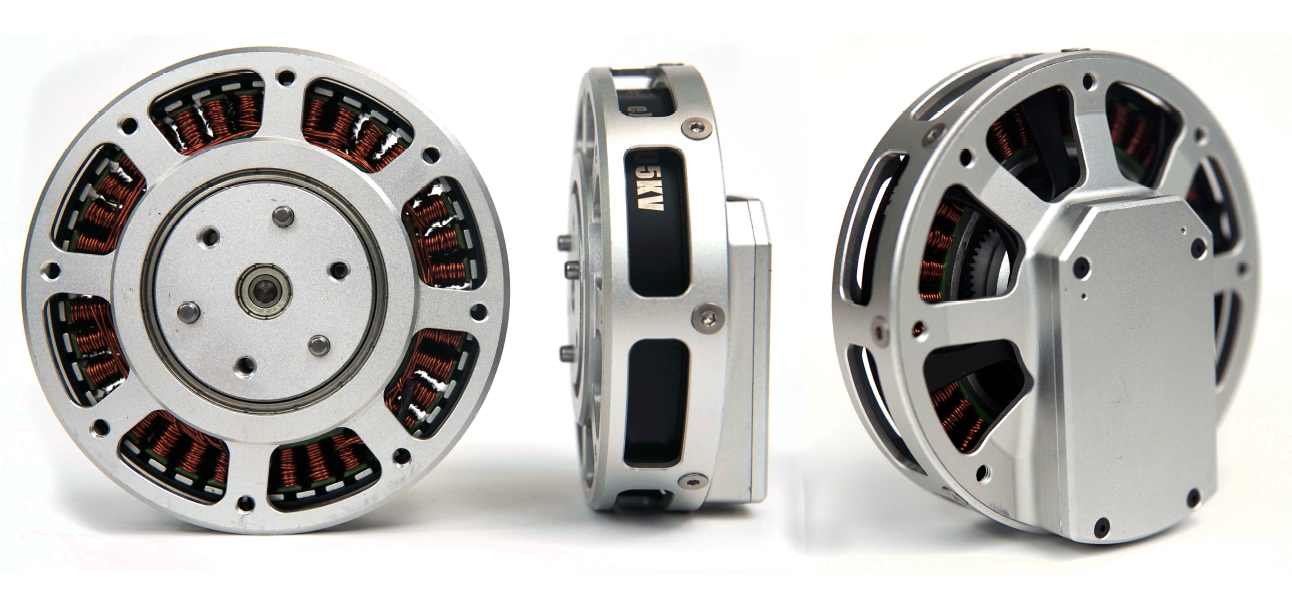
\includegraphics[width=0.6\columnwidth]{images/mini_cheetah_actuator}
\par\end{centering}
}
\par\end{centering}
\begin{centering}
\subfloat[Mini Cheetah Actuator Cross-Sectional View]{\begin{centering}
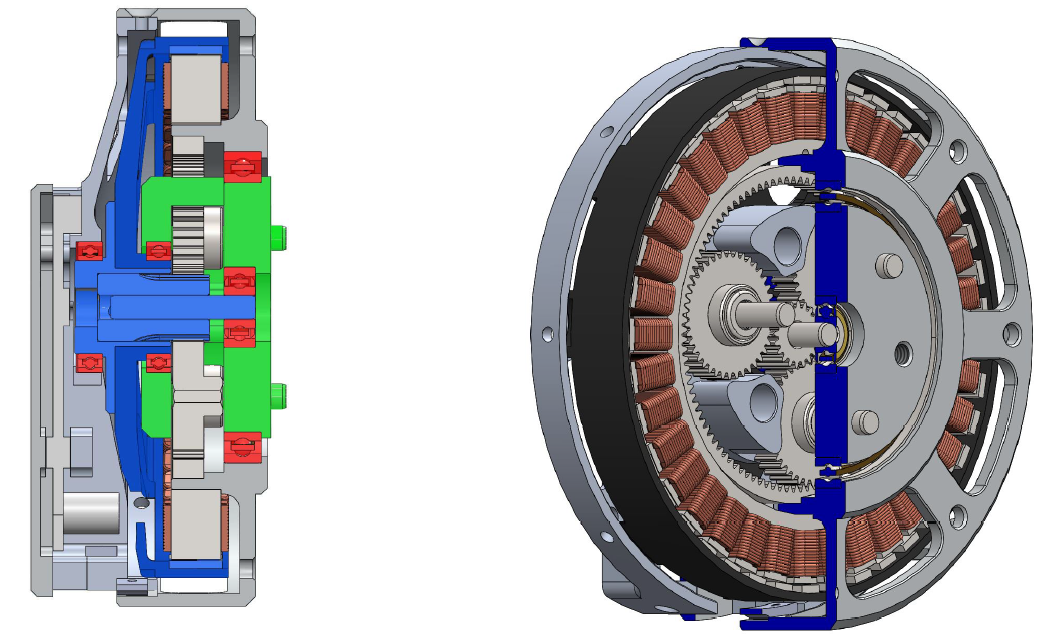
\includegraphics[width=0.5\columnwidth]{images/mini_cheetah_actuator_xsection}
\par\end{centering}
}
\par\end{centering}
\caption{Articulated Leg Configurations\label{fig:mini-cheetah-actuator}}
\end{figure}

Levine's OpenTorque is an open-source proprioceptive actuator with 3D-printed housing and transmission \cite{opentorque}. It uses an off-the-shelf brushless DC motor coupled to a single-stage planetary gearbox with a gear reduction ratio of 8. This provides a highly capable actuator with backdrivability while maintaining relatively low-cost and mechanical simplicity. An exploded view of OpenTorque is shown in Figure \ref{fig:opentorque}.

\begin{figure}[H]
\begin{centering}
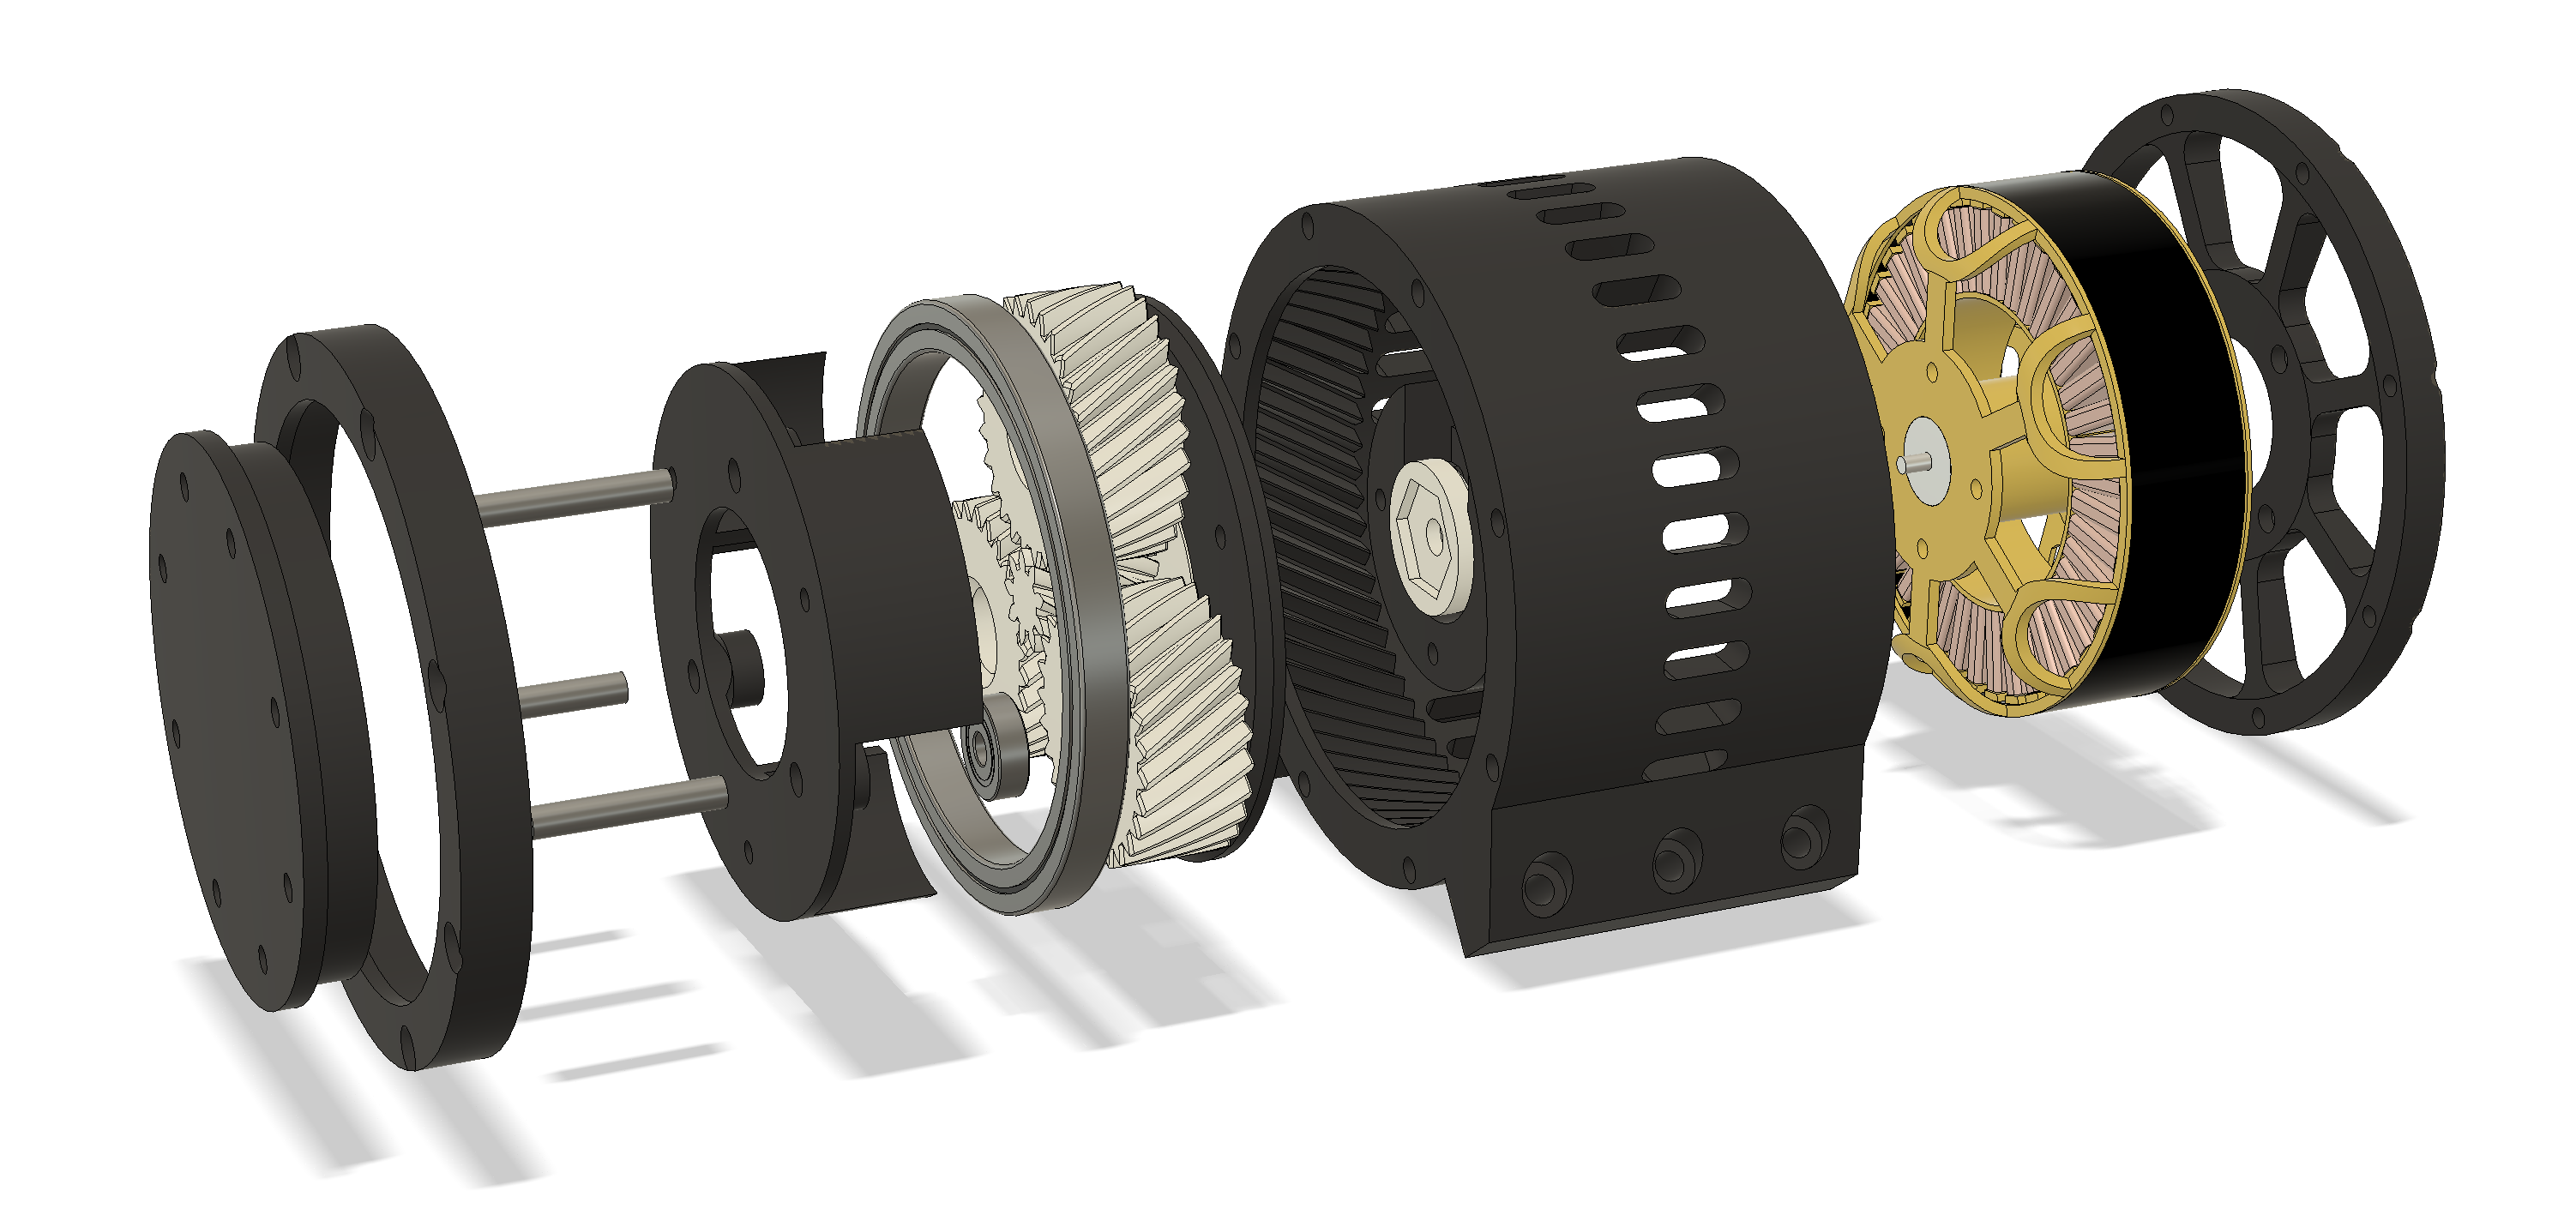
\includegraphics[width=0.8\columnwidth]{images/opentorque}
\par\end{centering}
\caption{OpenTorque Exploded View\label{fig:opentorque}}
\end{figure}

Hydraulic actuators provide high force density and impact robustness without adding significant mass and inertia to its legs. However, they have complicated closed-loop control and are highly inefficient compared to electric motors. Series-elastic actuators uses series elastic springs connected to a high-torque electric motor to achieve high-frequency impact force filtering and energy storage for locomotion. However, they introduce mechanical complexity, require several positional sensors, and poor high-frequency control bandwidth. Proprioceptive actuators provide an ideal solution to legged locomotion with its high torque density electric motor coupled to a transmission with low gear reduction ratios. This allows them to achieve high output torques with high bandwidths and high backdrivability for impact mitigation. Therefore, this project will use a proprioceptive actuator topology patterned after the Mini Cheetah actuator and OpenTorque.

\section{Mechanical Legs}

The next most important part of a quadrupedal robot are its mechanical legs. Their design and topology determines the overall performance and behavior of the robot since these define its effective maneuverability, walking speed, and load capacity \cite{designprinciples}. There are three types of mechanical legs that are commonly used by quadrupeds: prismatic, articulated, and redundant articulated legs. 

Prismatic legs are the simplest type of mechanical legs since they only have a single rotating joint and a prismatic joint as shown in Figure \ref{fig:prismatic-leg} \cite{quadrobotlegs}. 

\begin{figure}[H]
\begin{centering}
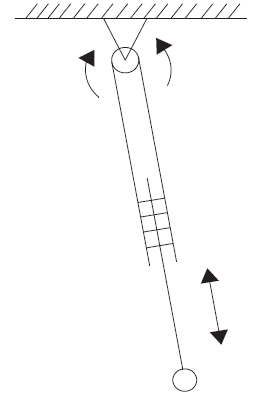
\includegraphics[width=0.3\columnwidth]{images/prismatic_leg}
\par\end{centering}
\caption{Prismatic Leg Topology\label{fig:prismatic-leg}}
\end{figure}

This type of leg typically mimics the bounce and compliance of an animal's leg with its prismatic joint using different kinds of springs. The work of Raibert et al. used a hydraulic actuator that is in series with an air spring, shown in Figure \ref{fig:quad-running-robot}, to control the leg length while still having compliance from the spring \cite{quadrunningrobot}. The Scout II quadrupedal robot, made by Poulakakis et al., uses only passive springs in its design for its prismatic legs which is shown in Figure \ref{fig:scout-ii} \cite{quadrobotlegs, scoutii}.

\begin{figure}[H]
\begin{centering}
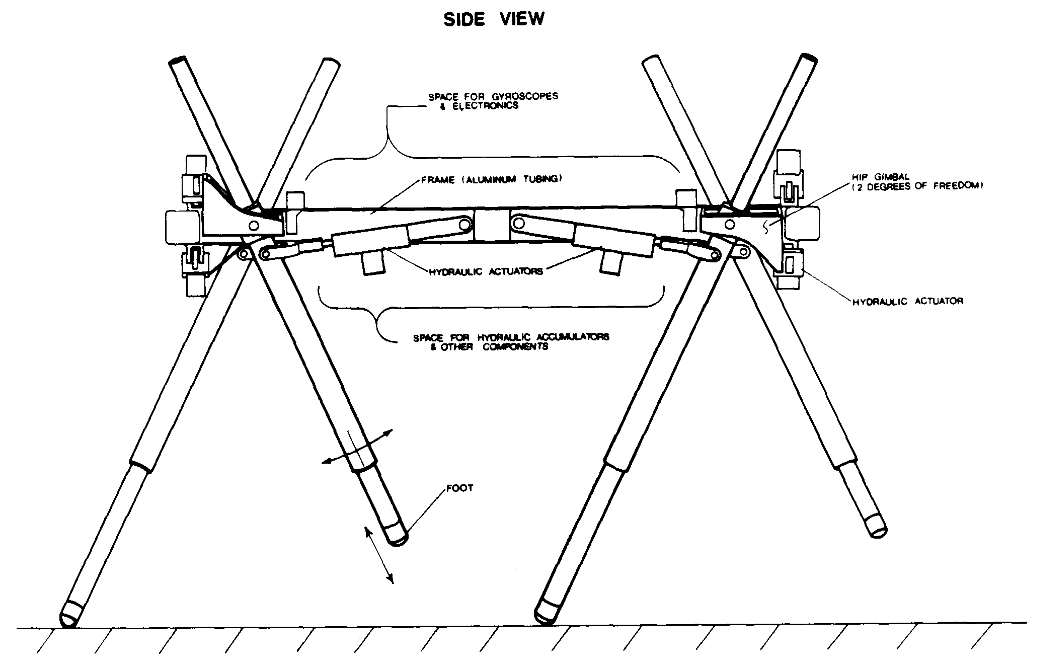
\includegraphics[width=0.75\columnwidth]{images/quad_running_robot}
\par\end{centering}
\caption{Four-legged Running Machine\label{fig:quad-running-robot}}
\end{figure}

\begin{figure}[H]
\begin{centering}
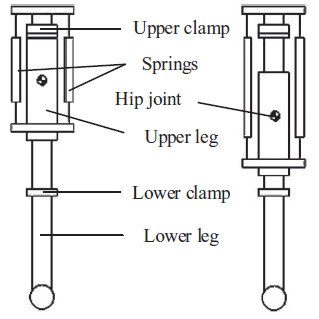
\includegraphics[width=0.3\columnwidth]{images/scout_ii}
\par\end{centering}
\caption{Scout II Robot\label{fig:scout-ii}}
\end{figure}

Prismatic legs are lightweight and have low inertia which is ideal for high-speed locomotion. Due to some designs using passive spring systems, less energy has to be expended to actuate the legs therefore high-efficiency movement can be achieved. They are also innately impact-resistant and provide fixed compliance to outside forces acting on it.

The second type of mechanical legs is the articulated leg. This leg topology replaces the prismatic joint of the prismatic leg with a rotational joint, similar to a knee or elbow joint, giving it a total of two rotational joints. This topology is a better representation, compared to the prismatic leg, of a typical leg structure of a natural four-legged animal. Control of the leg length is done by actuation of each rotational joint in conjunction with each other. The topology of the leg joints is shown in Figure \ref{fig:articulated-leg} \cite{quadrobotlegs}. 

\begin{figure}[H]
\begin{centering}
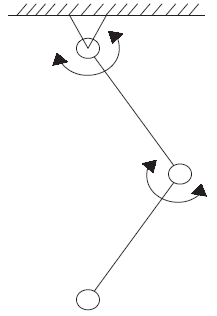
\includegraphics[width=0.3\columnwidth]{images/articulated_leg}
\par\end{centering}
\caption{Articulated Leg Topology\label{fig:articulated-leg}}
\end{figure}

There are two types of configuration of articulated legs on a quadruped: mammal and sprawling configuration. Mammal configurations have their legs positioned vertically with respect to the robot while sprawling configuration have the first segment of the leg (thigh) positioned horizontally with respect to the robot and the second leg segment (shank) is oriented vertically. The topologies of both configurations are shown in Figure \ref{fig:articulated-configurations} \cite{titanxiii}.

\begin{figure}[H]
\begin{centering}
\subfloat[Mammal Configuration]{\begin{centering}
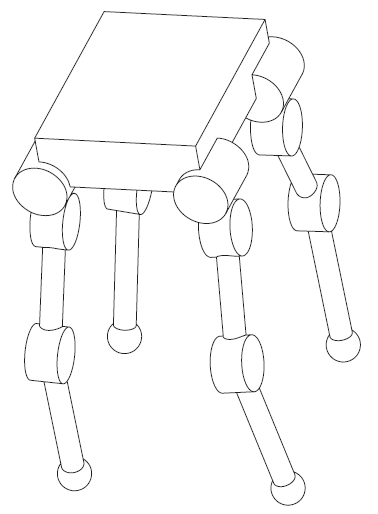
\includegraphics[width=0.25\columnwidth]{images/mammal_articulated}
\par\end{centering}
}
\par\end{centering}
\begin{centering}
\subfloat[Sprawling Configuration]{\begin{centering}
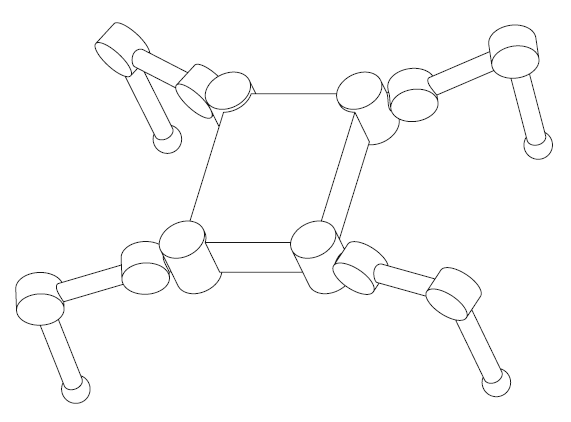
\includegraphics[width=0.4\columnwidth]{images/sprawling_articulated}
\par\end{centering}
}
\par\end{centering}
\caption{Articulated Leg Configurations\label{fig:articulated-configurations}}
\end{figure}

Mammal configurations are often more compact and have a smaller footprint, with the added benefit of requiring low joint torques with the legs bent. On the other hand, sprawling configurations are typically more stable due to its large stability polygon and its ability to lower its center of gravity without affecting its locomotion. This configuration, however, has several disadvantages compared to the mammal configuration. Sprawling configurations require the pitch axis to continuously generate torque to support its own weight, therefore reducing its efficiency. They also move significantly slower than mammal configurations.

Semini et al. have developed three quadrupedal robots with articulated legs, namely: HyQ, HyQ2Max, and MiniHyQ. The HyQ quadrupedal robot uses electro-hydraulic actuated legs. This system combines the high torque output of hydraulic actuators with the space-efficiency and high-speed of electric actuators to provide high power-to-weight ratio, high actuation speed, and torque robustness. The thigh of the robot is composed of parallel ribs that are linked together, keeping it lightweight and maintaining low inertia. The shank is a cylindrical structure that houses an additional passive prismatic ankle joint. The topology of the HyQ robot leg is shown in Figure \ref{fig:hyq-leg} \cite{quadrobotlegs, hyq}.

\begin{figure}[H]
\begin{centering}
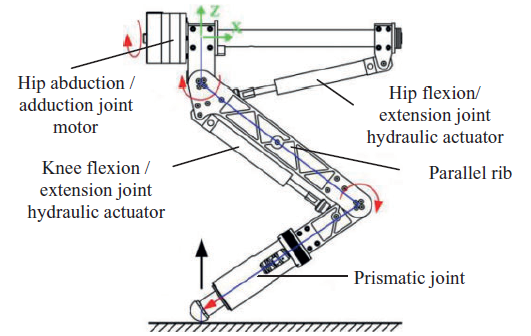
\includegraphics[width=0.7\columnwidth]{images/hyq}
\par\end{centering}
\caption{HyQ Leg Topology\label{fig:hyq-leg}}
\end{figure}

The HyQ2Max quadrupedal robot builds upon the HyQ with higher joint torques and payload, faster movement, and wider range of motion while maintaining the use of hydraulic actuators \cite{hyq2max}. The MiniHyQ quadrupedal robot builds upon the previous two models. Despite the name, it has the same leg length as the HyQ but with less weight and higher range of motion. The leg topology of the MiniHyQ is shown in Figure \ref{fig:mini-hyq-leg} \cite{minihyq}.

\begin{figure}[H]
\begin{centering}
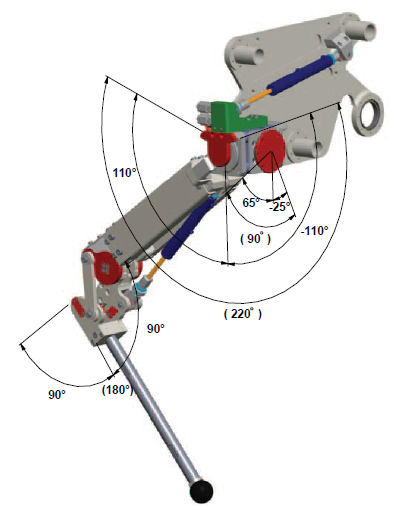
\includegraphics[width=0.3\columnwidth]{images/minihyq}
\par\end{centering}
\caption{MiniHyQ Leg Topology\label{fig:mini-hyq-leg}}
\end{figure}

The ANYmal quadrupedal robot is designed for operation in harsh environments. It stands at 0.5 m tall with leg lengths of 0.28 m and a weight of approximately 30 kg. It uses highly integrated modular SEAs, called ANYdrive, to drive each joint in a mammalian configuration. The leg links of the robot are built with offsets to allow the joints to fully rotate which enables the robot to have a wide range of motion and mobility. The ANYmal is able to use its limbs above its body, like hands, for tasks such as opening doors. The knee joint actuators, however, are mounted on the leg which increases the leg's inertia. The topology of the ANYmal is shown in Figure \ref{fig:anymal} \cite{anymal, anymal2}.

\begin{figure}[H]
\begin{centering}
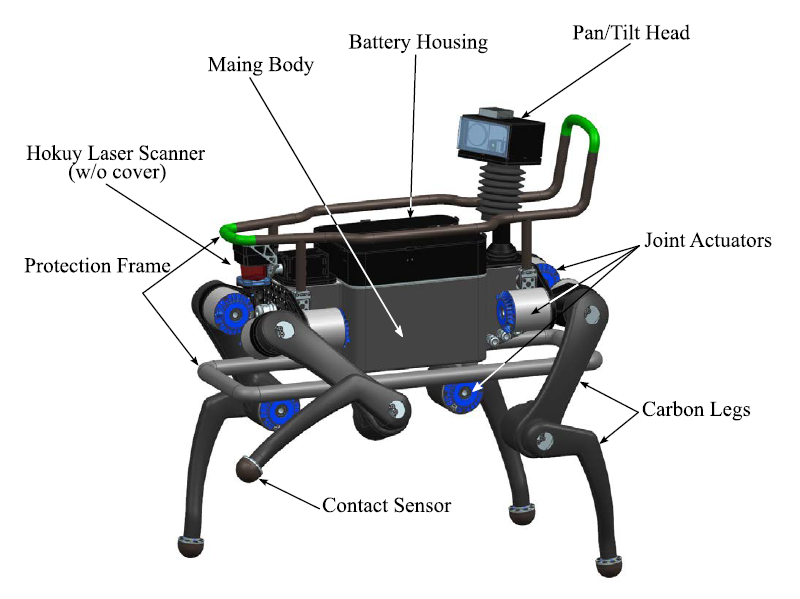
\includegraphics[width=0.7\columnwidth]{images/anymal}
\par\end{centering}
\caption{ANYmal Topology\label{fig:anymal}}
\end{figure}

The MIT Cheetah 3 is a highly efficient quadrupedal robot designed for high-speed locomotion. It can stand up to 0.88 m tall with leg lengths of 0.34 m and a weight of approximately 45 kg. The robot uses proprioceptive actuators mounted on its hips and close to its body to minimize the weight and inertia of its legs. The hip abduction/adduction and flexion/extension joints are quasi-direct driven while the knee flexion/extension is timing belt driven due to the actuator being away from the joint. The topology of the Cheetah 3 is shown in Figure \ref{fig:cheetah-3-leg} \cite{mitcheetah3}.

\begin{figure}[H]
\begin{centering}
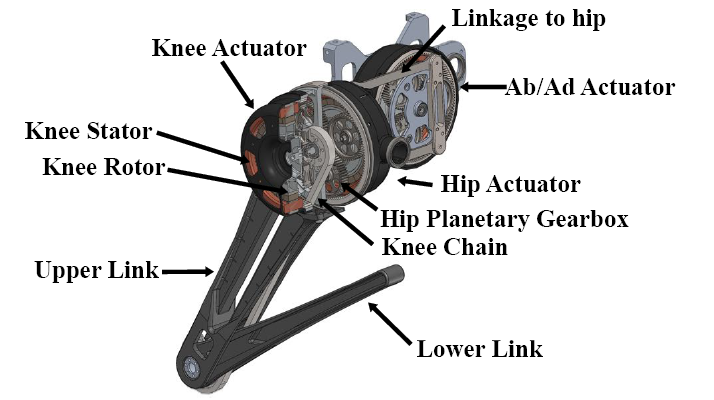
\includegraphics[width=0.7\columnwidth]{images/cheetah_3}
\par\end{centering}
\caption{Cheetah 3 Leg Topology\label{fig:cheetah-3-leg}}
\end{figure}

The third and last type of mechanical legs to be discussed is the redundant articulated leg. This leg topology simply takes an articulated leg and adds at least one more rotating joint. This mimics leg structurs of animals with toes or hoofs and provide better kinematic properties when traversing rugged terrain. The leg topology is shown in Figure \ref{fig:redundant-articulated-leg} \cite{quadrobotlegs}.

\begin{figure}[H]
\begin{centering}
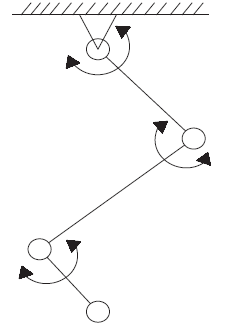
\includegraphics[width=0.3\columnwidth]{images/redundant_articulated_leg}
\par\end{centering}
\caption{Redundant Articulated Leg Topology\label{fig:redundant-articulated-leg}}
\end{figure}

MIT's Cheetah and Cheetah 2 are quadrupedal robots with redundant articulated legs. Both quadrupedal robots employ proprioceptive actuators to drive the joints. The knee joint is driven by a parallel linkage mechanisim connected to the actuator while the ankle only has a passive linkage mechanism which mimics the motion of the Achilles tendon. The topology of the Cheetah and Cheetah 2 robots are shown in Figure \ref{fig:cheetah12-leg} \cite{quadrobotlegs, cheetah}.

\begin{figure}[H]
\begin{centering}
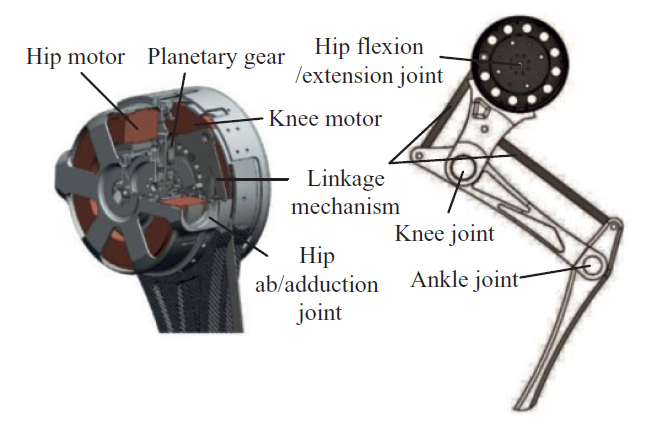
\includegraphics[width=0.6\columnwidth]{images/cheetah12}
\par\end{centering}
\caption{Cheetah and Cheetah 2 Leg Topology\label{fig:cheetah12-leg}}
\end{figure}

The use of prismatic legs, with its single rotating and prismatic joint, simplifies the control aspect and choice of hardware for the robot. It is also has the lowest weight and inertia of the three leg topologies discussed. However, the kinematics of the robot is greatly limited due to having fewer rotating joints. Redundant articulated legs, on the other hand, have the best kinematic performance, stability, workspace, and is the closest representation of natural toed or hoofed animals. However, it comes with the cost of adding actuators to control at least three rotational joints and adding complexity to the control aspect for the robot. Articulated legs strike a middle-ground with high maneuverability and stability while having fewer actuators than redundant articulated legs. With that being said, the articulated leg topology, patterned after the Cheetah 3, will be used throughout the project.

\section{Materials}

Fused Deposition Modeling (FDM) 3D-printing is a low-cost rapid prototyping method that enables easy manufacturing of complex geometry with high strength. It involves melting of thermoplastic material through an extrusion nozzle and depositing them layer-by-layer to eventually form a solid shape \cite{pla-composites}. The three most used materials, and the ones to be discussed, are polylactic acid (PLA), acrylonitrile butadiene styrene (ABS), and polyethylene terephthalate glycol-modified (PETG). 

PLA is one of the most widely used material for 3D-printing because of its ease-of-use, high availability, and affordability. It is known for its low thermal conductivity, high toughness, and bio-degradability \cite{plaabships}. PLA, however, has a lower melting point meaning it does not perform well in heated conditions.

ABS is also one of the most widely used material for 3D-printing. It is known for its low thermal conductivity, high tougness, and high impact resistance \cite{plaabships}. In contrast to PLA, ABS has a higher melting point and is heat resistant, making it suitable for operation in heated conditions. However, it is harder to use because of its higher temperature requirements and its tendency to warp while printing.

PETG is gaining popularity in the 3D-printing department because it combines the ease-of-use of PLA with the impact- and heat-resistance of ABS. It shares the same strength characteristics of ABS along with its high melting point. Additionally, PETG does not warp while printing. However, PETG is more expensive than both PLA and ABS.

Tensile, flexural, and impact strengths of PopBit T-PLA and T-ABS taken from their respective datasheets, which are attached in Appendix A \cite{tpla, tabs}, are listed in Table \ref{tab:material-strengths}.

\begin{table}[H]
\caption{Tensile and Flexural Strengths of T-PLA and T-ABS\label{tab:material-strengths}}

\centering{}
\begin{tabular}{|c|c|c|c|}
\hline 
Material & Tensile Strength (MPa) & Flexural Strength (MPa) & Impact Strength\tabularnewline
\hline 
\hline 
PLA & 32.2 $\pm$ 1.3 & 57 $\pm$ 2.2 & 14.1 $\pm$ 1.1 \tabularnewline
\hline 
ABS & 34 $\pm$ 1.3 & 70.6 $\pm$ 3.1 & 10.8 $\pm$ 0.8 \tabularnewline
\hline 
\hline 
\end{tabular}
\end{table}

As shown, PLA has a marginally lower tensile strength compared to ABS but falls behind in flexural strength. PLA, however, has higher impact strength than ABS. PLA is chosen to be used in this project due to its overall close strength to ABS and it is much easier to print. PETG is a strong alternative for when more strength and heat-resistance is needed.

\section{Control}

Essential to any legged robot is its manner of locomotion. Different configurations of the mechanical legs and type of actuator require different approaches to gait and stability control. 

\begin{figure}[H]
\begin{centering}
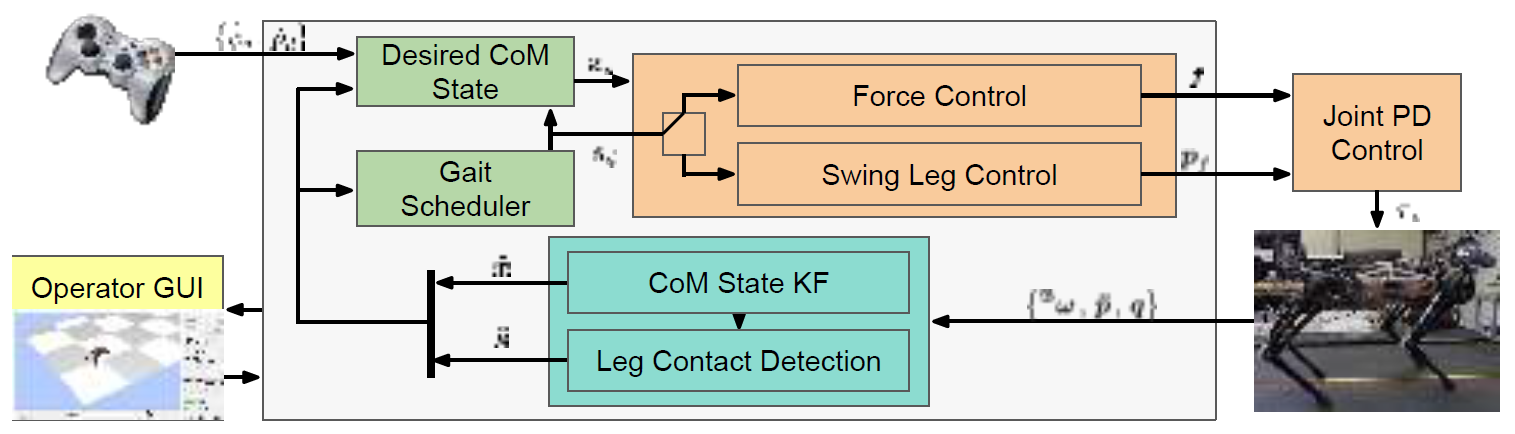
\includegraphics[width=0.8\columnwidth]{images/cheetah3_control}
\par\end{centering}
\caption{MIT Cheetah 3 Control Block Diagram\label{fig:cheetah3-control}}
\end{figure}

The Cheetah 3 employs the control system shown in block diagram form in Figure \ref{fig:cheetah3-control} \cite{mitcheetah3}. The Cheetah 3 takes in a desired translational velocity and turning rate from the operator and uses them to plan the trajectory for the center-of-mass (CoM) of the robot. The trajectory is then sent to the body and leg controllers to generate the necessary force commands for each leg depending on whether it is in a stance or swing state. The controller uses a linear relationship of the robot's CoM translational $\ddot{\mathbf{p}}_c$ and body angular acceleration $\dot{\mathbf{\omega}}_b$ with the forces $\mathbf{F} = {(\mathbf{F}_1^T, \mathbf{F}_2^T, \mathbf{F}_3^T, \mathbf{F}_4^T)}^T$ as shown in Equation \ref{eq:controller-model} \cite{balancecontroller}.

\begin{equation}
    \label{eq:controller-model}
    \begin{bmatrix}
        \mathbf{I}_3 & \cdots & \mathbf{I}_3 \\
        [\mathbf{p}_1 - \mathbf{p}_c]\times & \cdots & [\mathbf{p}_4 - \mathbf{p}_c]\times \\
    \end{bmatrix}
    \mathbf{F}
    =
    \begin{bmatrix}
        m(\ddot{\mathbf{p}}_c + \mathbf{g}) \\
        \mathbf{I}_G \dot{\mathbf{\omega}}_b
    \end{bmatrix}
\end{equation}

Where $m$ is the robot's mass, $\mathbf{I}_G$ is the robot's centroidal inertia, $g$ is the gravity vector, and $\mathbf{p}_i$ are the positions of the feet. The Cheetah 3 also implements a balance controller that uses Proportional-Derivative (PD) control on the CoM and body orientation. The cost function for this controller chooses a balance between driving the CoM to the desired state, minimizing forces used, and penalizing deviations between the current and previous time frames. The gaits of the Cheetah 3 are defined by event-based finite state machines that schedule the nominal contact and swing phases. This allows easy modifications to the gaits and their transitions. A virtual support polygon is defined by the robot to provide a desired CoM position across different gaits. The algorithm biases away from legs that are about to swing and towards legs nearing touchdown allowing for the maintaning of forward momentum during locomotion.

\cleardoublepage{}

\chapter{Problem Statement and Objectives \label{cha:ProbStatement}}

Legged robots have been the topic of countless research in past years. Due to their high maneuverability and flexibility, they are able to operate in rough environments in contrast to wheeled robots. Being able to carry large payloads through rough terrain makes them ideal for disaster response operations. Recent developments have even allowed these robots to react to their environment without the need for computer vision through proprioception.

These robots, however, are far too expensive for academic experimental and research purposes. Even the smaller, albeit newer, robust implementations still cost a few thousands of US dollars at least. 

In line with this, the project aims to develep a prototype of a cost-efficient 12-DOF quadrupedal robot. It would have the ability to react to its surroundings using proprioceptive actuators with custom joint controllers and off-the-shelf brushless DC motors.

The project also aims to provide the Robotics Automation Laboratory with a robust platform that can be used for future development of legged robotics.

\cleardoublepage{}

\chapter{Methodology\label{cha:Methodology}}

\section{Design and Implementation}
\subsection{Mechanical}

The quadrupedal robot implements three Degrees of Freedom (DOF) per leg. Two DOF joints are used for the hips which control the abduction/adduction and flexion/extension motion. One DOF joints are used for the knee to control its flexion/extension motion. No joints are designed into the quadruped's ankles since the actuators are backdrivable and force-compliant.  Fusion360 is used to design and simulate the quadruped. The 3D model of the robot is shown in Figure \ref{fig:open-cauchy}.

\begin{figure}[H]
\begin{centering}
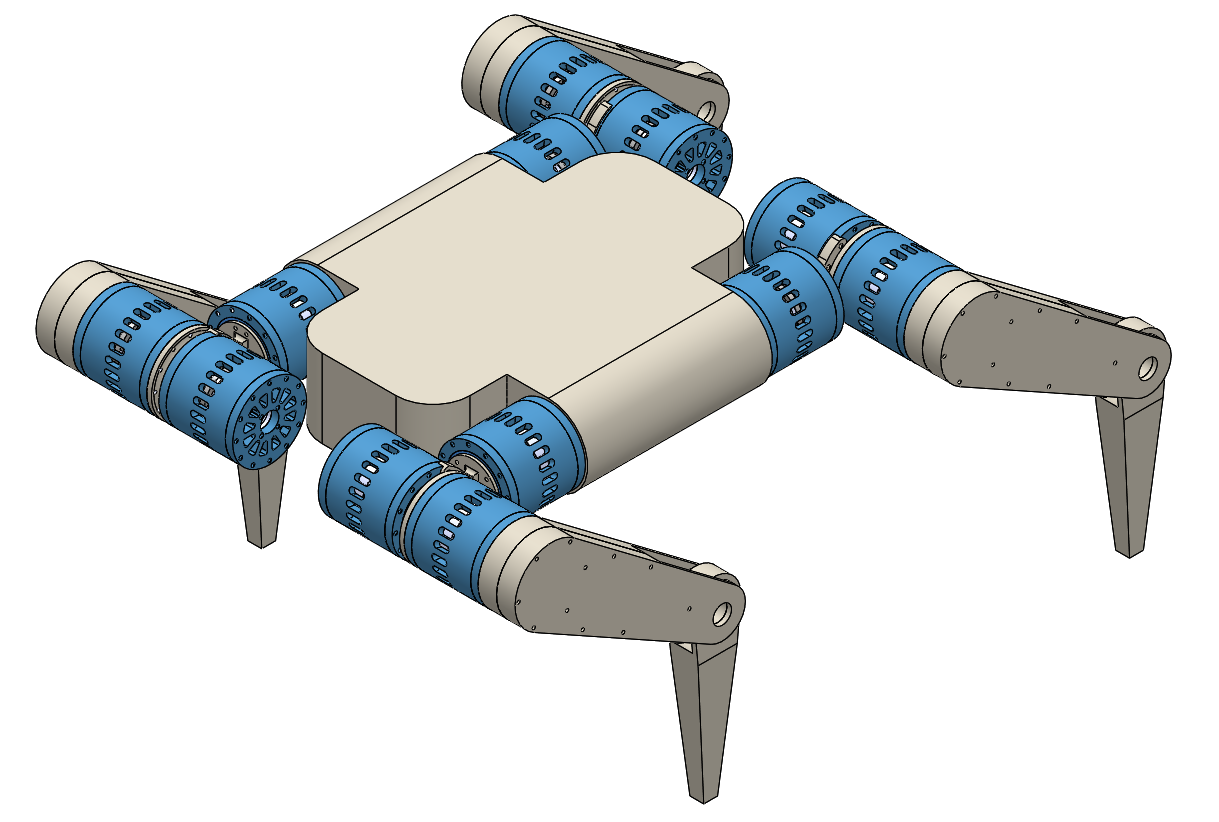
\includegraphics[width=0.7\columnwidth]{images/open_cauchy}
\par\end{centering}
\caption{Quadrupedal Robot 3D Model\label{fig:open-cauchy}}
\end{figure}

Each joint will be driven by an actuator that consists of a BLDC motor coupled to a single state planetary gearbox. The planetary gearbox has a reduction ratio of 6.125 which makes the actuator quasi-direct drive and allows for force compliancy and proprioception. Each actuator including the planetary gearbox will be 3D printed using readily available tough polylactic acid (T-PLA) from PopBit. Bearings are added to provide smoother rotation of gears and more even distribution of loads, while threaded inserts are used to have stronger points to screw on. The actuator has an overall diameter of 110 mm and length of 75 mm and weighs 700 grams in total. The 3D model of the joint actuator is shown in Figure \ref{fig:joint-actuator}.

\begin{figure}[H]
\begin{centering}
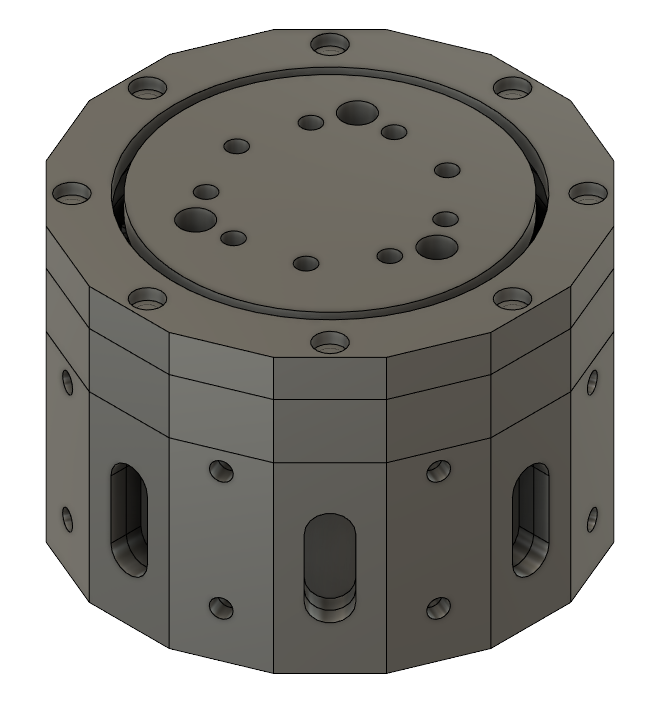
\includegraphics[width=0.5\columnwidth]{images/joint_actuator}
\par\end{centering}
\caption{Joint Actuator 3D Model\label{fig:joint-actuator}}
\end{figure}

The three joint actuators for each leg are designed to be mounted at the top of the legs and as close to the body as possible. This makes sure that the actual legs would be as light as possible to minimize the leg's inertia. The two hip joints are directly coupled to the actuator using a 3D printed joint connector. The knee joint, on the other hand, uses a timing belt coupled to the output of the knee actuator to control the knee, providing an additional 1.25 gear reduction ratio. This configuration allows the robot's hips to have 180 degrees of rotation about its own roll axis and 360 degrees about its pitch axis. The robot's knees have 270 degrees of rotation. 

The quadruped's legs consists of two links: upper and lower link. The upper link consists of two halves, connected to each other using screws, to enable access to the timing belt during assembly and maintenance. The lower link is one solid part that has a gear at one of its end and revolves around the lower part of the upper link. Lastly, the foot is a round object made out of rubber to absorb small amount of forces and provide some compliance. The lengths of each link is shown in Table \ref{tab:link-lengths}.

\begin{table}[H]
\caption{Leg Link Lengths\label{tab:link-lengths}}

\centering{}
\begin{tabular}{|c|c|}
\hline 
Link & Length (mm)\tabularnewline
\hline 
\hline 
Upper & 250\tabularnewline
\hline 
Lower & 200\tabularnewline
\hline 
\hline 
\end{tabular}
\end{table}

The hip abduction/adduction actuators are mounted onto the 3D printed body. The body houses the main controller of the robot and the battery to power the robot. The overall size of the quadrupedal robot is around 550 by 400 mm.

\subsection{Electronics}

The quadrupedal robot uses a custom designed joint controller and main controller board. The joint controller is responsible with controlling the brushless DC (BLDC) motor in the actuator while the main controller is responsible with trajectory generation and propagation of positional data for the joints. Both controller boards are designed around Microchip's dsPIC33CK family of digital signal controllers (DSCs). The specific model and features of the DSCs used are shown in Table \ref{tab:dspic-specs}.

\begin{table}[H]
\caption{dsPIC33K Model and Features\label{tab:dspic-specs}}

\centering{}
\begin{tabular}{|c|c|}
\hline 
dsPIC33CK128MP505 & dsPIC33CK128MP508\tabularnewline
\hline 
\hline 
48 Pins & 80 Pins\tabularnewline
\hline 
\multicolumn{2}{|c|}{8 PWM Pairs}\tabularnewline
\hline 
\multicolumn{2}{|c|}{High-Speed ADC}\tabularnewline
\hline 
\multicolumn{2}{|c|}{4-Wire SPI}\tabularnewline
\hline 
\multicolumn{2}{|c|}{UART}\tabularnewline
\hline 
\multicolumn{2}{|c|}{CAN-FD}\tabularnewline
\hline 
\hline 
\end{tabular}
\end{table}

The joint controller is made up of four main compontents: microcontroller, gate driver, output stage, and encoder. The microcontroller used is the dsPIC33CK128MP505. The gate driver used is Texas Instruments' DR8323 Three-Phase Smart Gate Driver. This gate driver is responsible for driving an external three-phase inverter stage that generates the sinusoidal voltages used to drive the motor. The three-phase inverter stage uses the N-channel NTMFS4935NT1G MOSFETs which are rated for 30V and 13A. Lastly, the controller uses an AS5047P magnetic rotary position sensor, that is mounted at the back of the printed circuit board (PCB), to sense the rotation of the BLDC rotor and track its position and speed with 14 bits of resolution. Shunt resistors are  added onto the board in order to measure the current in each phase of the motor. Other needed components such as resistors, capacitors, inductors, diodes, and terminals are also designed into the controller upon recommendation of each main components' datasheets. Schematic capture and PCB layout design for both the joint and main controller was done on KiCad. Top and bottom layers of the 2-layer joint controller PCB are shown in Figure \ref{fig:joint-controller}.

\begin{figure}[H]
\begin{centering}
\subfloat[Top Layer]{\begin{centering}
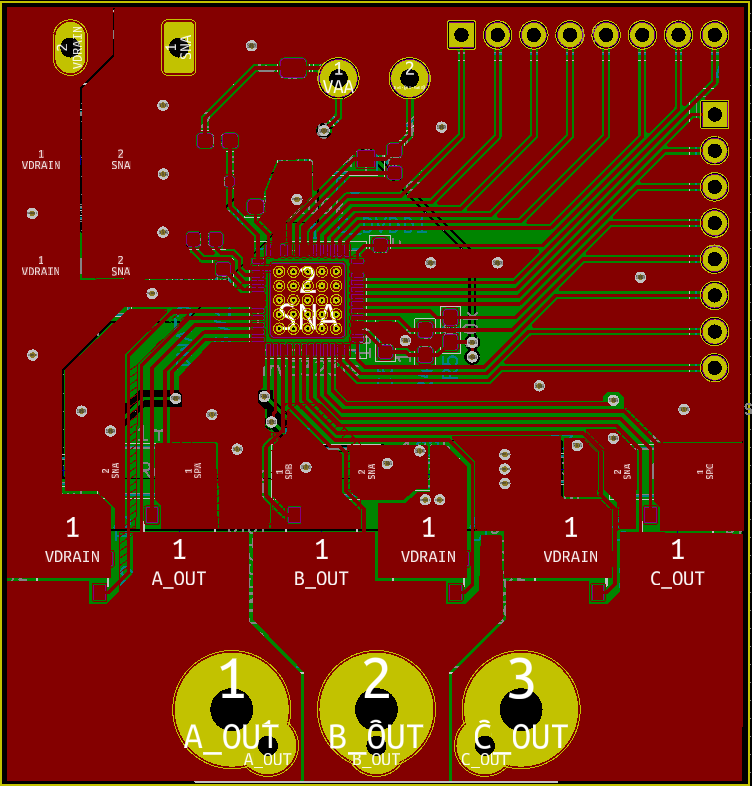
\includegraphics[width=0.4\columnwidth]{images/joint_controller_top}
\par\end{centering}
}
\par\end{centering}
\begin{centering}
\subfloat[Bottom Layer]{\begin{centering}
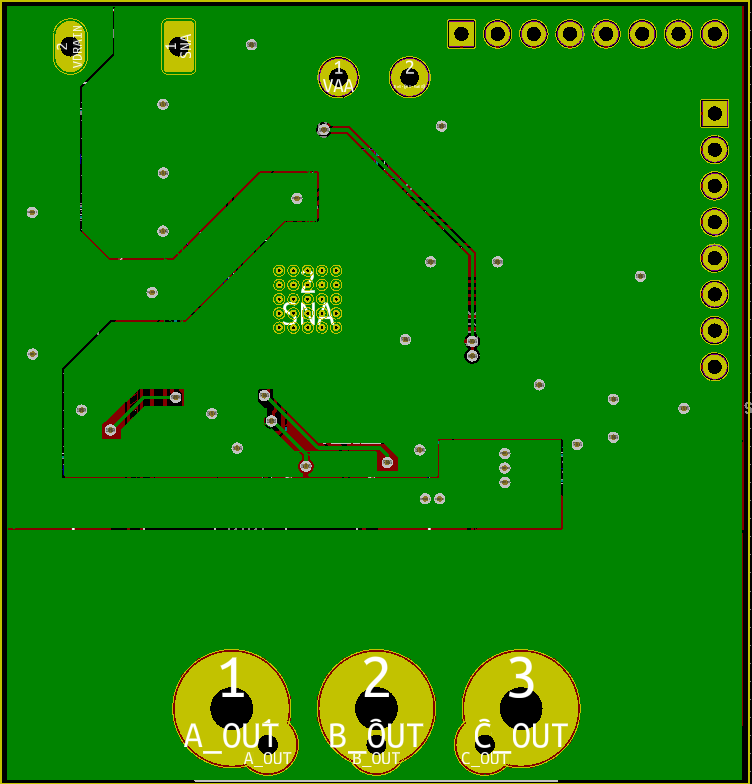
\includegraphics[width=0.4\columnwidth]{images/joint_controller_bottom}
\par\end{centering}
}
\par\end{centering}
\caption{Joint Controller PCB Design\label{fig:joint-controller}}
\end{figure}

The main controller is mainly composed of the dsPIC33CK128MP508 microcontroller. The board also features 12 terminals for the CAN bus connections of each actuator. UART breakout pins are also added for communication to a PC.

\subsection{Control}

Control in the quadrupedal robot can be divided into three parts: joint, stability, and gait control. Each part is independent but functions in conjuction with the others.

Joint control of the quadruped is distributed across the joint controllers of each actuator. It is responsible for controlling the torque and commutation of the BLDC motor in the actuator. It accepts positional data from the main controller and uses the Field Oriented Control (FOC) algorithm to generate three-phase sinusoidal voltages that maximize the torque output of the BLDC motor. The block diagram for the FOC algorithm is shown in Figure \ref{fig:foc-block-diagram} \cite{an1292}.

\begin{figure}[H]
\begin{centering}
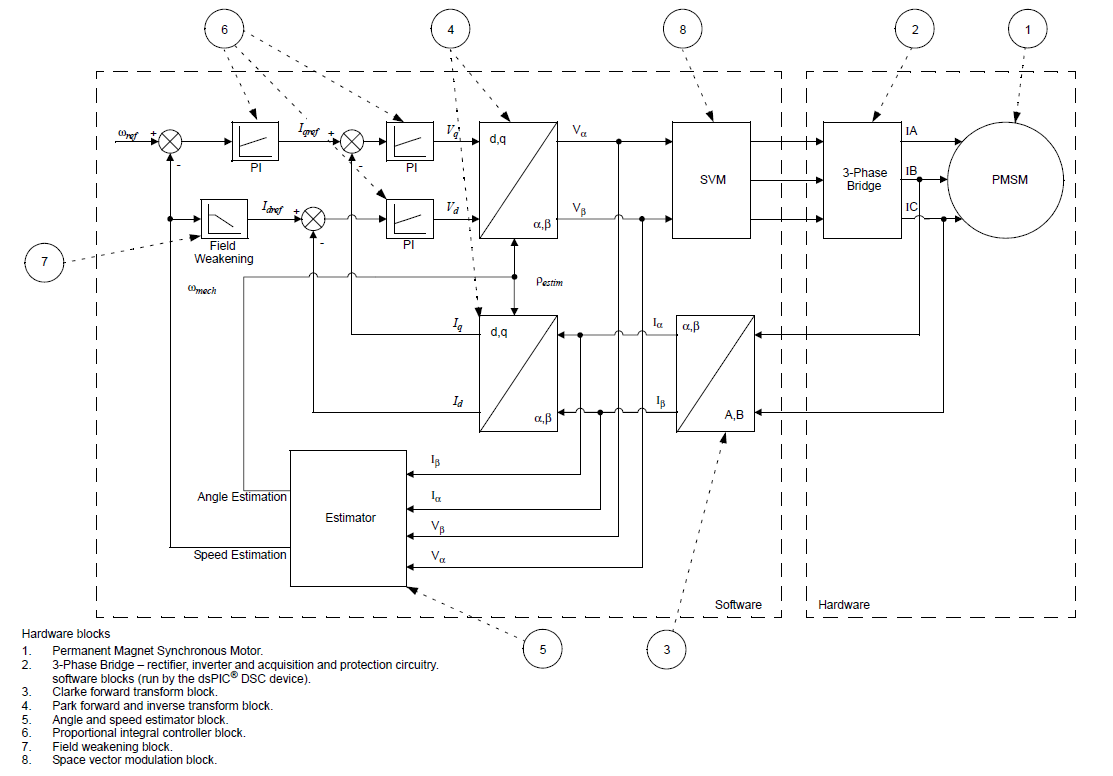
\includegraphics[width=1.0\columnwidth]{images/foc}
\par\end{centering}
\caption{Field-Oriented Control Block Diagram\label{fig:foc-block-diagram}}
\end{figure}

The first step in FOC is measuring the current of two phases of the motor and computing for the third using Equation \ref{eq:phase-currents}. 

\begin{equation} \label{eq:phase-currents}
    i_a + i_b + i_c = 0
\end{equation}

Clarke Transform, shown in Equation \ref{eq:clark-transform}, is applied to the three-phase currents that is referenced to the stator and moves them onto a 2D orthogonal system, still referenced to the stator, called alpha-beta.

\begin{equation} \label{eq:clark-transform}
    \begin{split}
        i_\alpha &= i_a \\
        i_\beta &= \frac{i_a + 2 i_b}{\sqrt{3}}
    \end{split}
\end{equation}

Park Transform, shown in Equation \ref{eq:park-transform}, is applied to the two-phase, stator-referenced currents and rotates them onto the d-q coordinate system that is referenced to the rotor. The two-phase currents are now treated as DC signals and can be controlled using conventional Proportional-Integral (PI) controllers. 

\begin{equation} \label{eq:park-transform}
    \begin{split}
        i_d &= i_\alpha \cos \theta + i_\beta \sin \theta \\
        i_q &= -i_\alpha \cos \theta + i_\beta \sin \theta 
    \end{split}
\end{equation}

Error signals are generated for the position, speed, Iq, and Id currents and are fed through individual cascaded PI controllers. The rotor angle and rotor speed are computed using phase-locked loop (PLL) estimator shown in Figure \ref{fig:pll-estimator} \cite{an1292}. 

\begin{figure}[H]
\begin{centering}
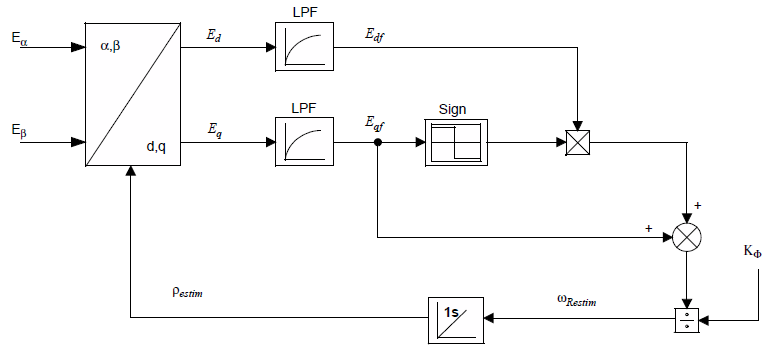
\includegraphics[width=1.0\columnwidth]{images/pll_estimator}
\par\end{centering}
\caption{PLL Estimator Block Diagram\label{fig:pll-estimator}}
\end{figure}

The Vq and Vd outputs from the respective Iq and Id PI controllers are then referenced back onto the stator using the Inverse Park Transform. 

The final step in FOC is to generate pulse-width modulation signals, with frequency of 20 kHz, for the three-phase inverter using Space Vector Modulation (SVM). SVM represent the six possible states of the three-phase inverter as space vectors which are 60 degrees apart. It calculates which sector the resultant voltage vector is in and achieves this voltage by varying, thus averaging, the time spent on the two adjacent space vector states. The duty cycles are calculated and updated. The algorithm is done every Analog-to-Digital Converter (ADC) interrupt which is triggered by the PWM module.

While the motor is being driven by the FOC algorithm, the rotor encoder continually tracks the position of the rotor. This feedback from the encoder is used for position control, on top of the torque and speed control, of the motor. The measured position is subtracted from the desired position, received from the main controller, and the error signal is fed to its separate PI controller. 

\section{Testing}

SPECIFY TARGET RESULTS

The actuator's torque output with varying current is to be tested by attaching a link with a length of 200 mm directly to its output carrier and measuring the maximum weight it can support without failure. The torque vs current is to be graphed alongside with the calculated torque constant. The actuator's thermal performance is to be tested by running the BLDC motor at its maximum rated speed for a set amount of time and measuring the temperature of the actuator using a thermal imaging camera or a thermocouple.

Tuning of the PI controllers is to be done empirically. For the FOC, the inner PI controllers are to be tuned first before the outer controllers. Step response of the joint actuators to torque, current, speed, and position set points are to be tested and verified. Testing of each leg is to be done before assembly of the quadruped. Static gaits is to be fed to the quadruped robot to test its initial stability.

\cleardoublepage{}
\chapter{Preliminary Findings\label{cha:Prelims}}

\section{Design}

\subsection{Mechanical}

The prototype of the 3D-printed actuator is shown in Figure \ref{fig:actuator-prototype}. It has a single stage planetary gearbox with 6.125 gear reduction ratio. It has 82 teeth on its ring gear, 32 on each of its three planetary gears, and 16 teeth on the sun gear that's directly attached to the motor with M3 screws. The actuator housing is held together by M4 screws. It weighs around 800 grams with the bearings.

\begin{figure}[H]
\begin{centering}
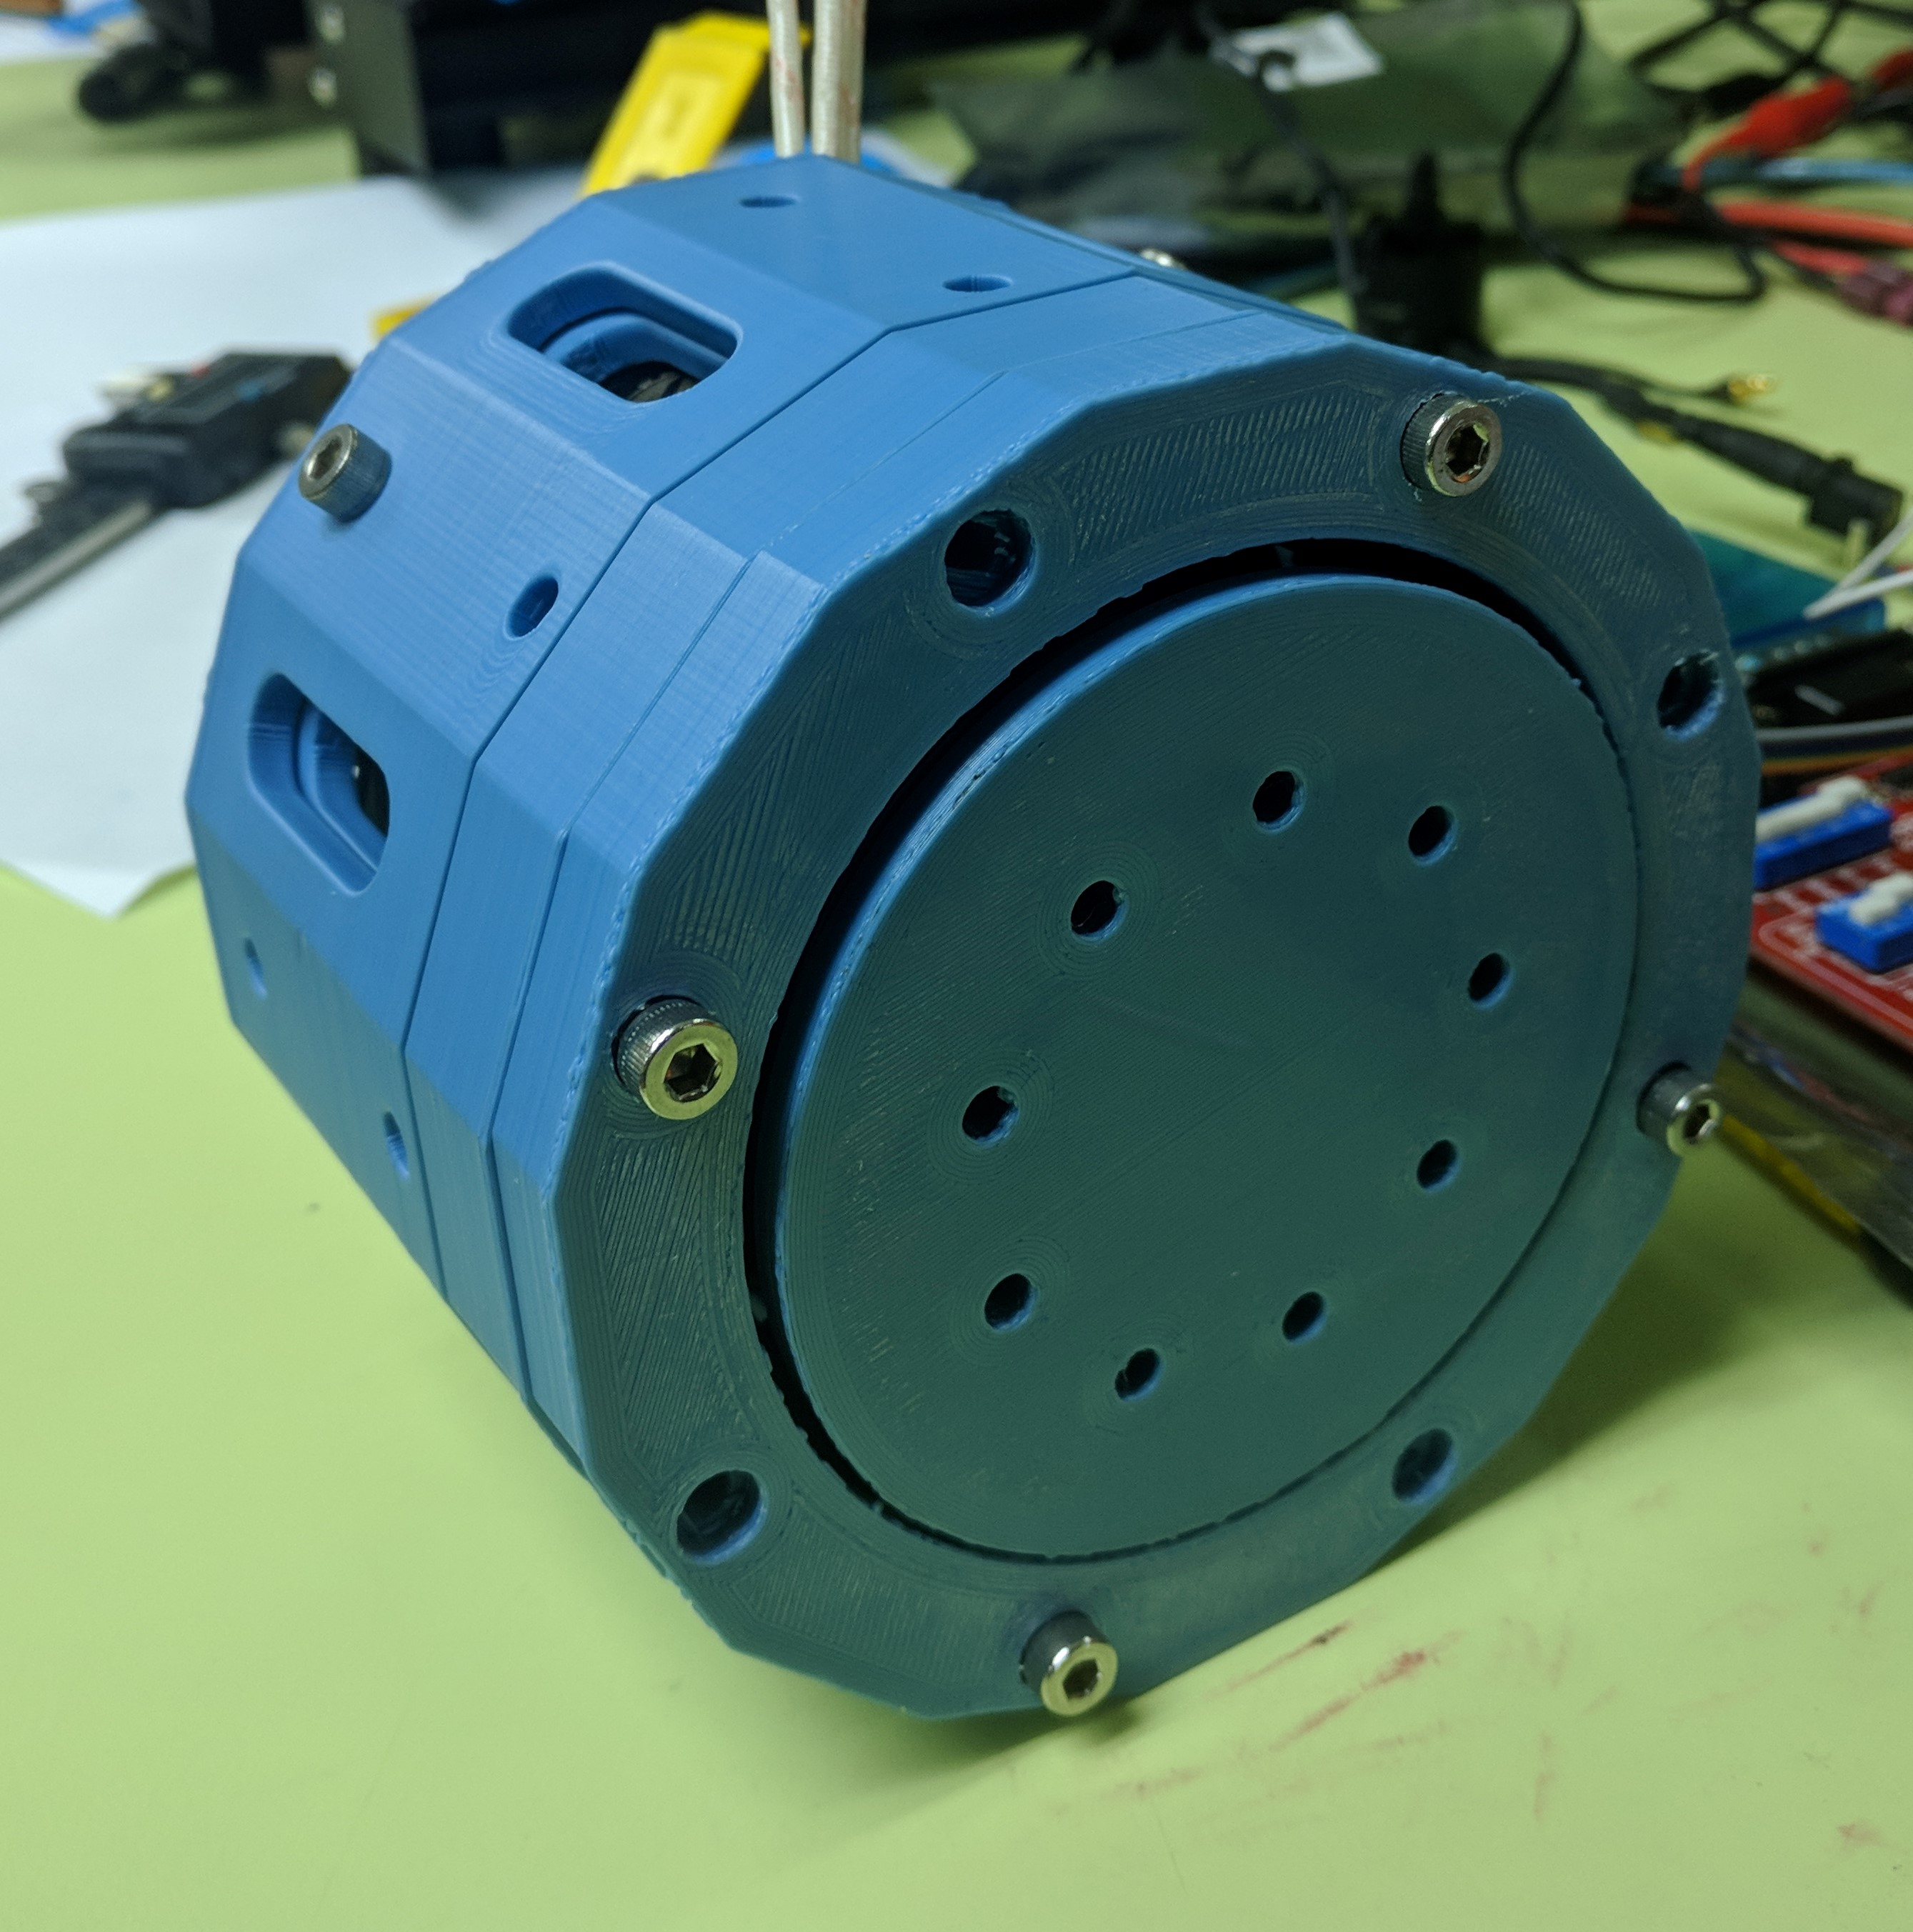
\includegraphics[width=0.5\columnwidth]{images/actuator_prototype}
\par\end{centering}
\caption{Actuator Prototype\label{fig:actuator-prototype}}
\end{figure}

The actuator uses a Herlea X8311s brushless DC motor procured from Alibaba. It has a diameter of 89.6 mm, length of 33.3 mm, weight of 388 g, and a KV rating of 140. The motor is shown in Figure \ref{fig:motor}.

\begin{figure}[H]
\begin{centering}
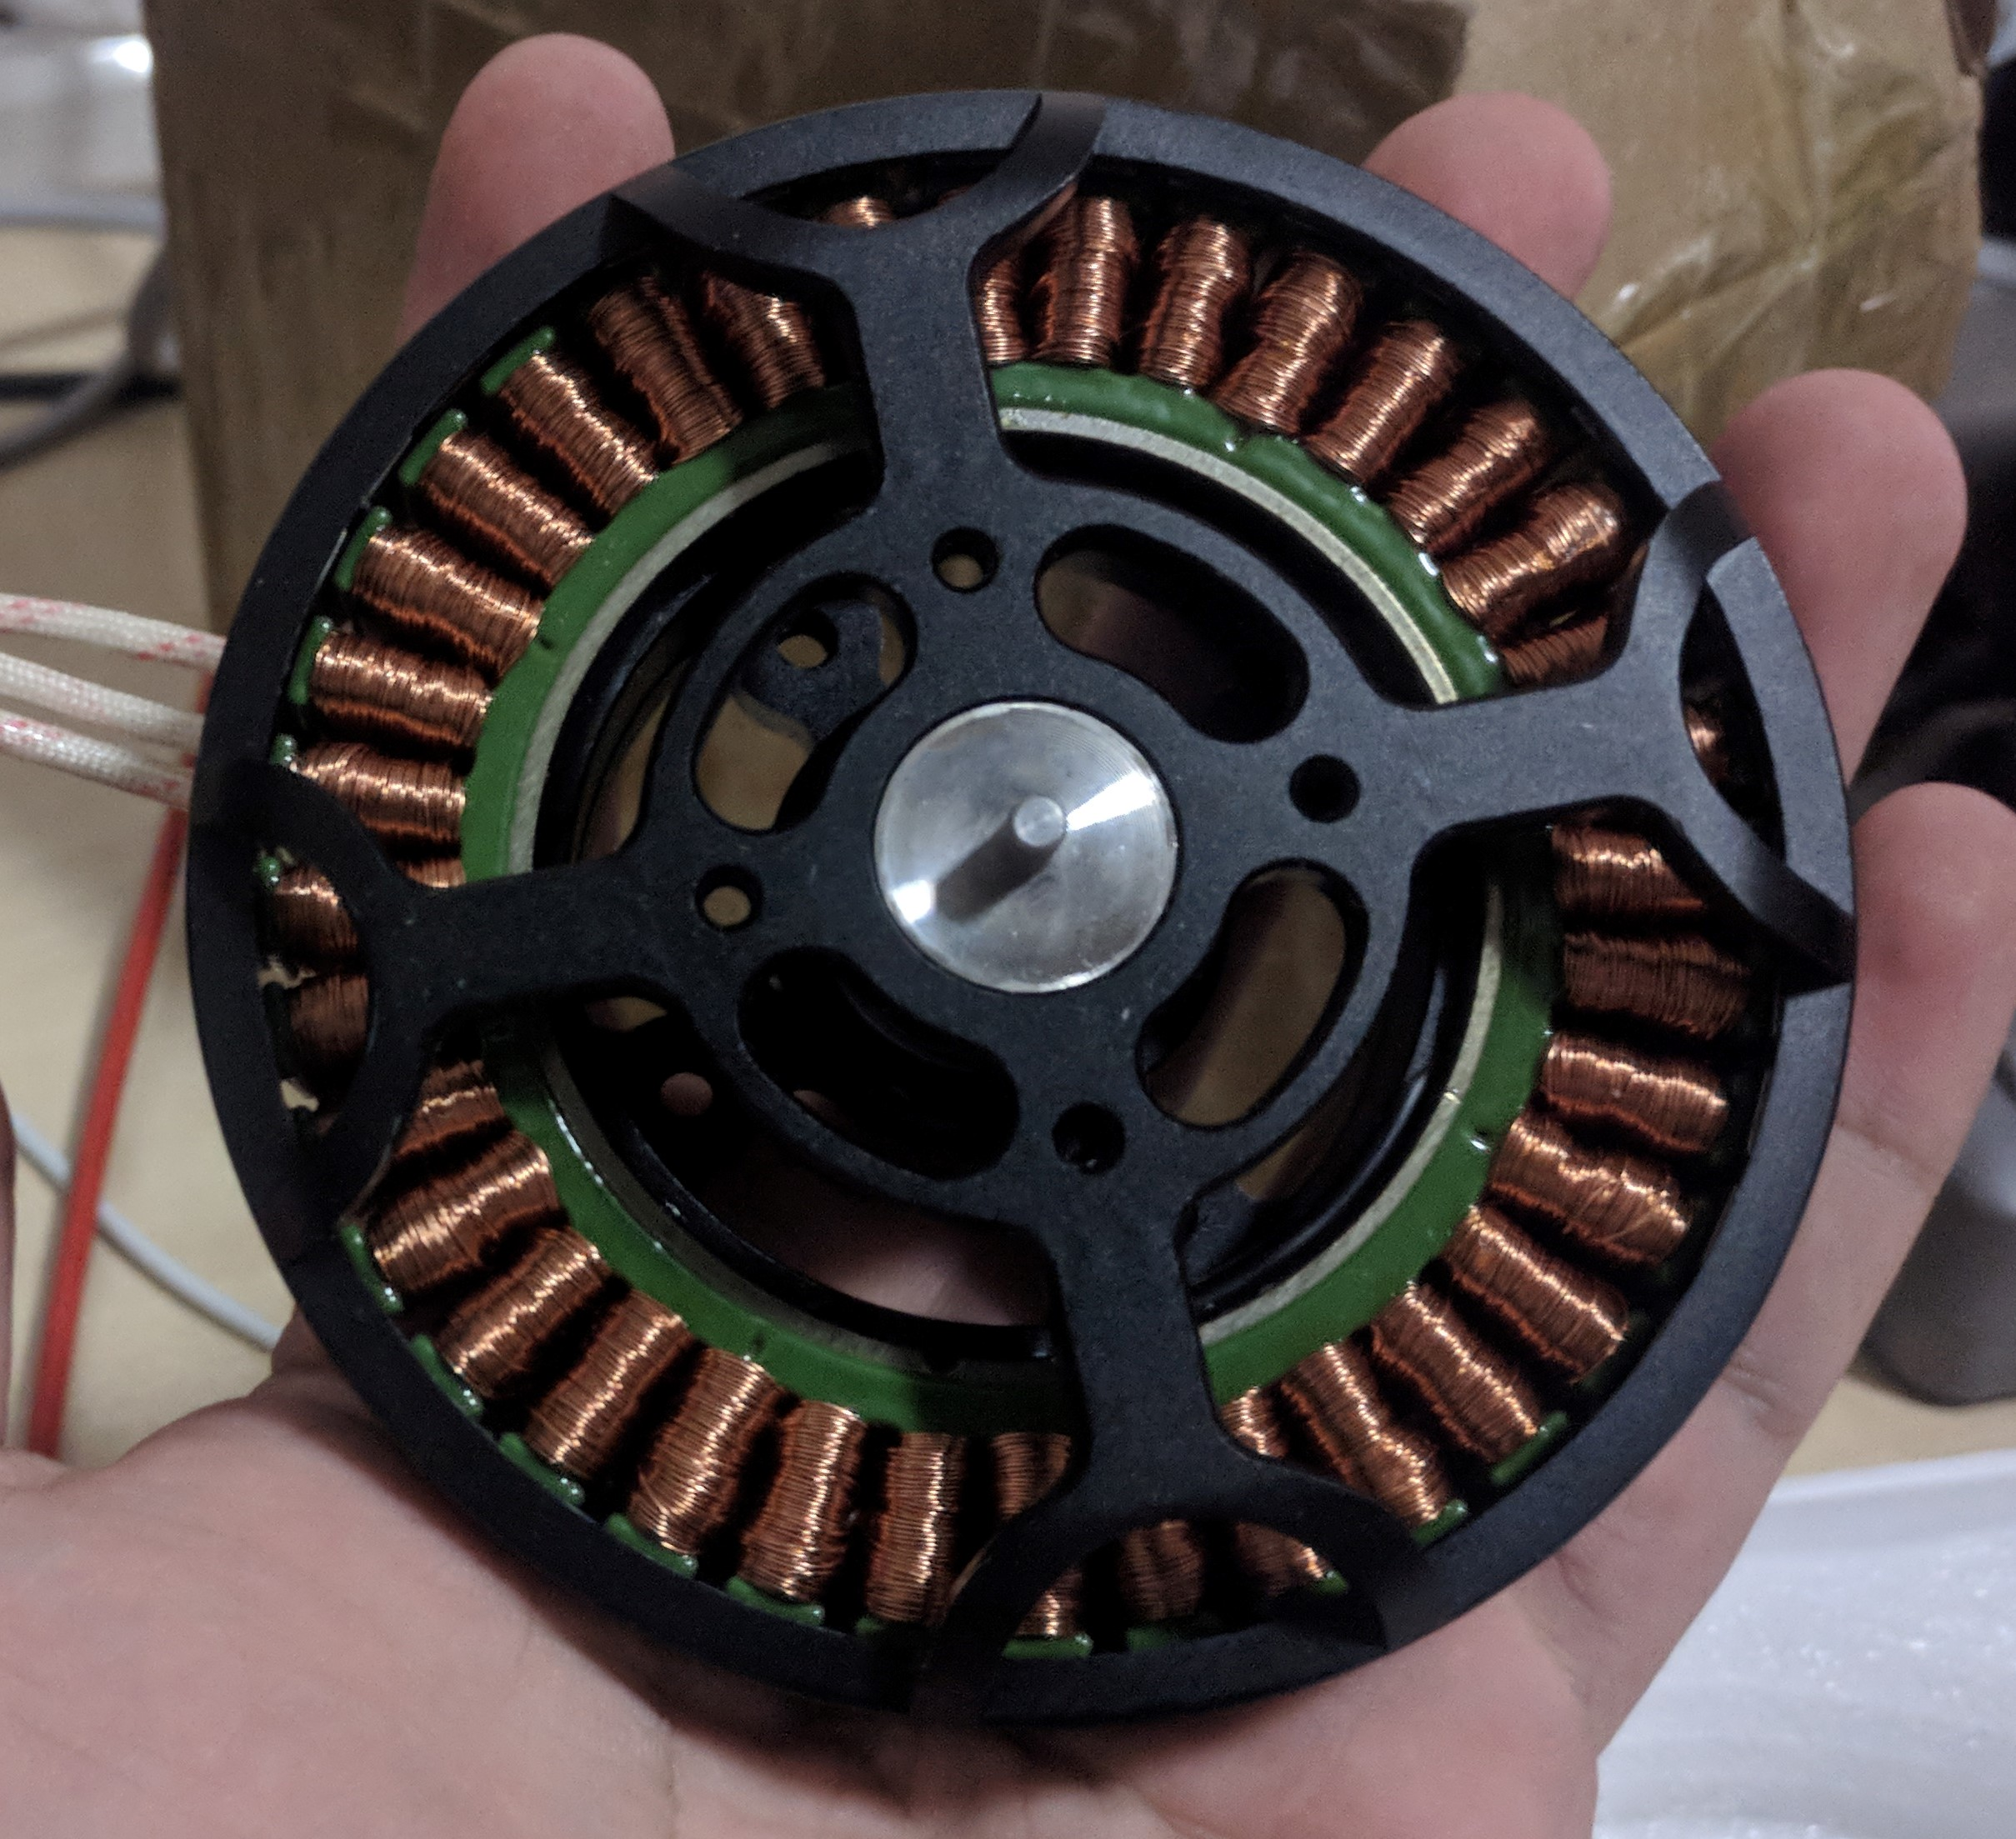
\includegraphics[width=0.5\columnwidth]{images/motor}
\par\end{centering}
\caption{Herlea X8311s Brushless DC Motor\label{fig:motor}}
\end{figure}

\subsection{Electronics}

The joint controller PCB fabrication is out-sourced to JLCPCB. It's overall size is 52.5 mm by 52.5 mm. The components for the joint controller is procured from Digi-Key. The PCB was put through a reflow oven to solder the components easily. The unpopulated and populated joint controller PCB are shown in Figures \ref{fig:joint-controller-pcb} and \ref{fig:joint-controller-pcb-full} respectively.

\begin{figure}[H]
\begin{centering}
\subfloat[Top Layer]{\begin{centering}
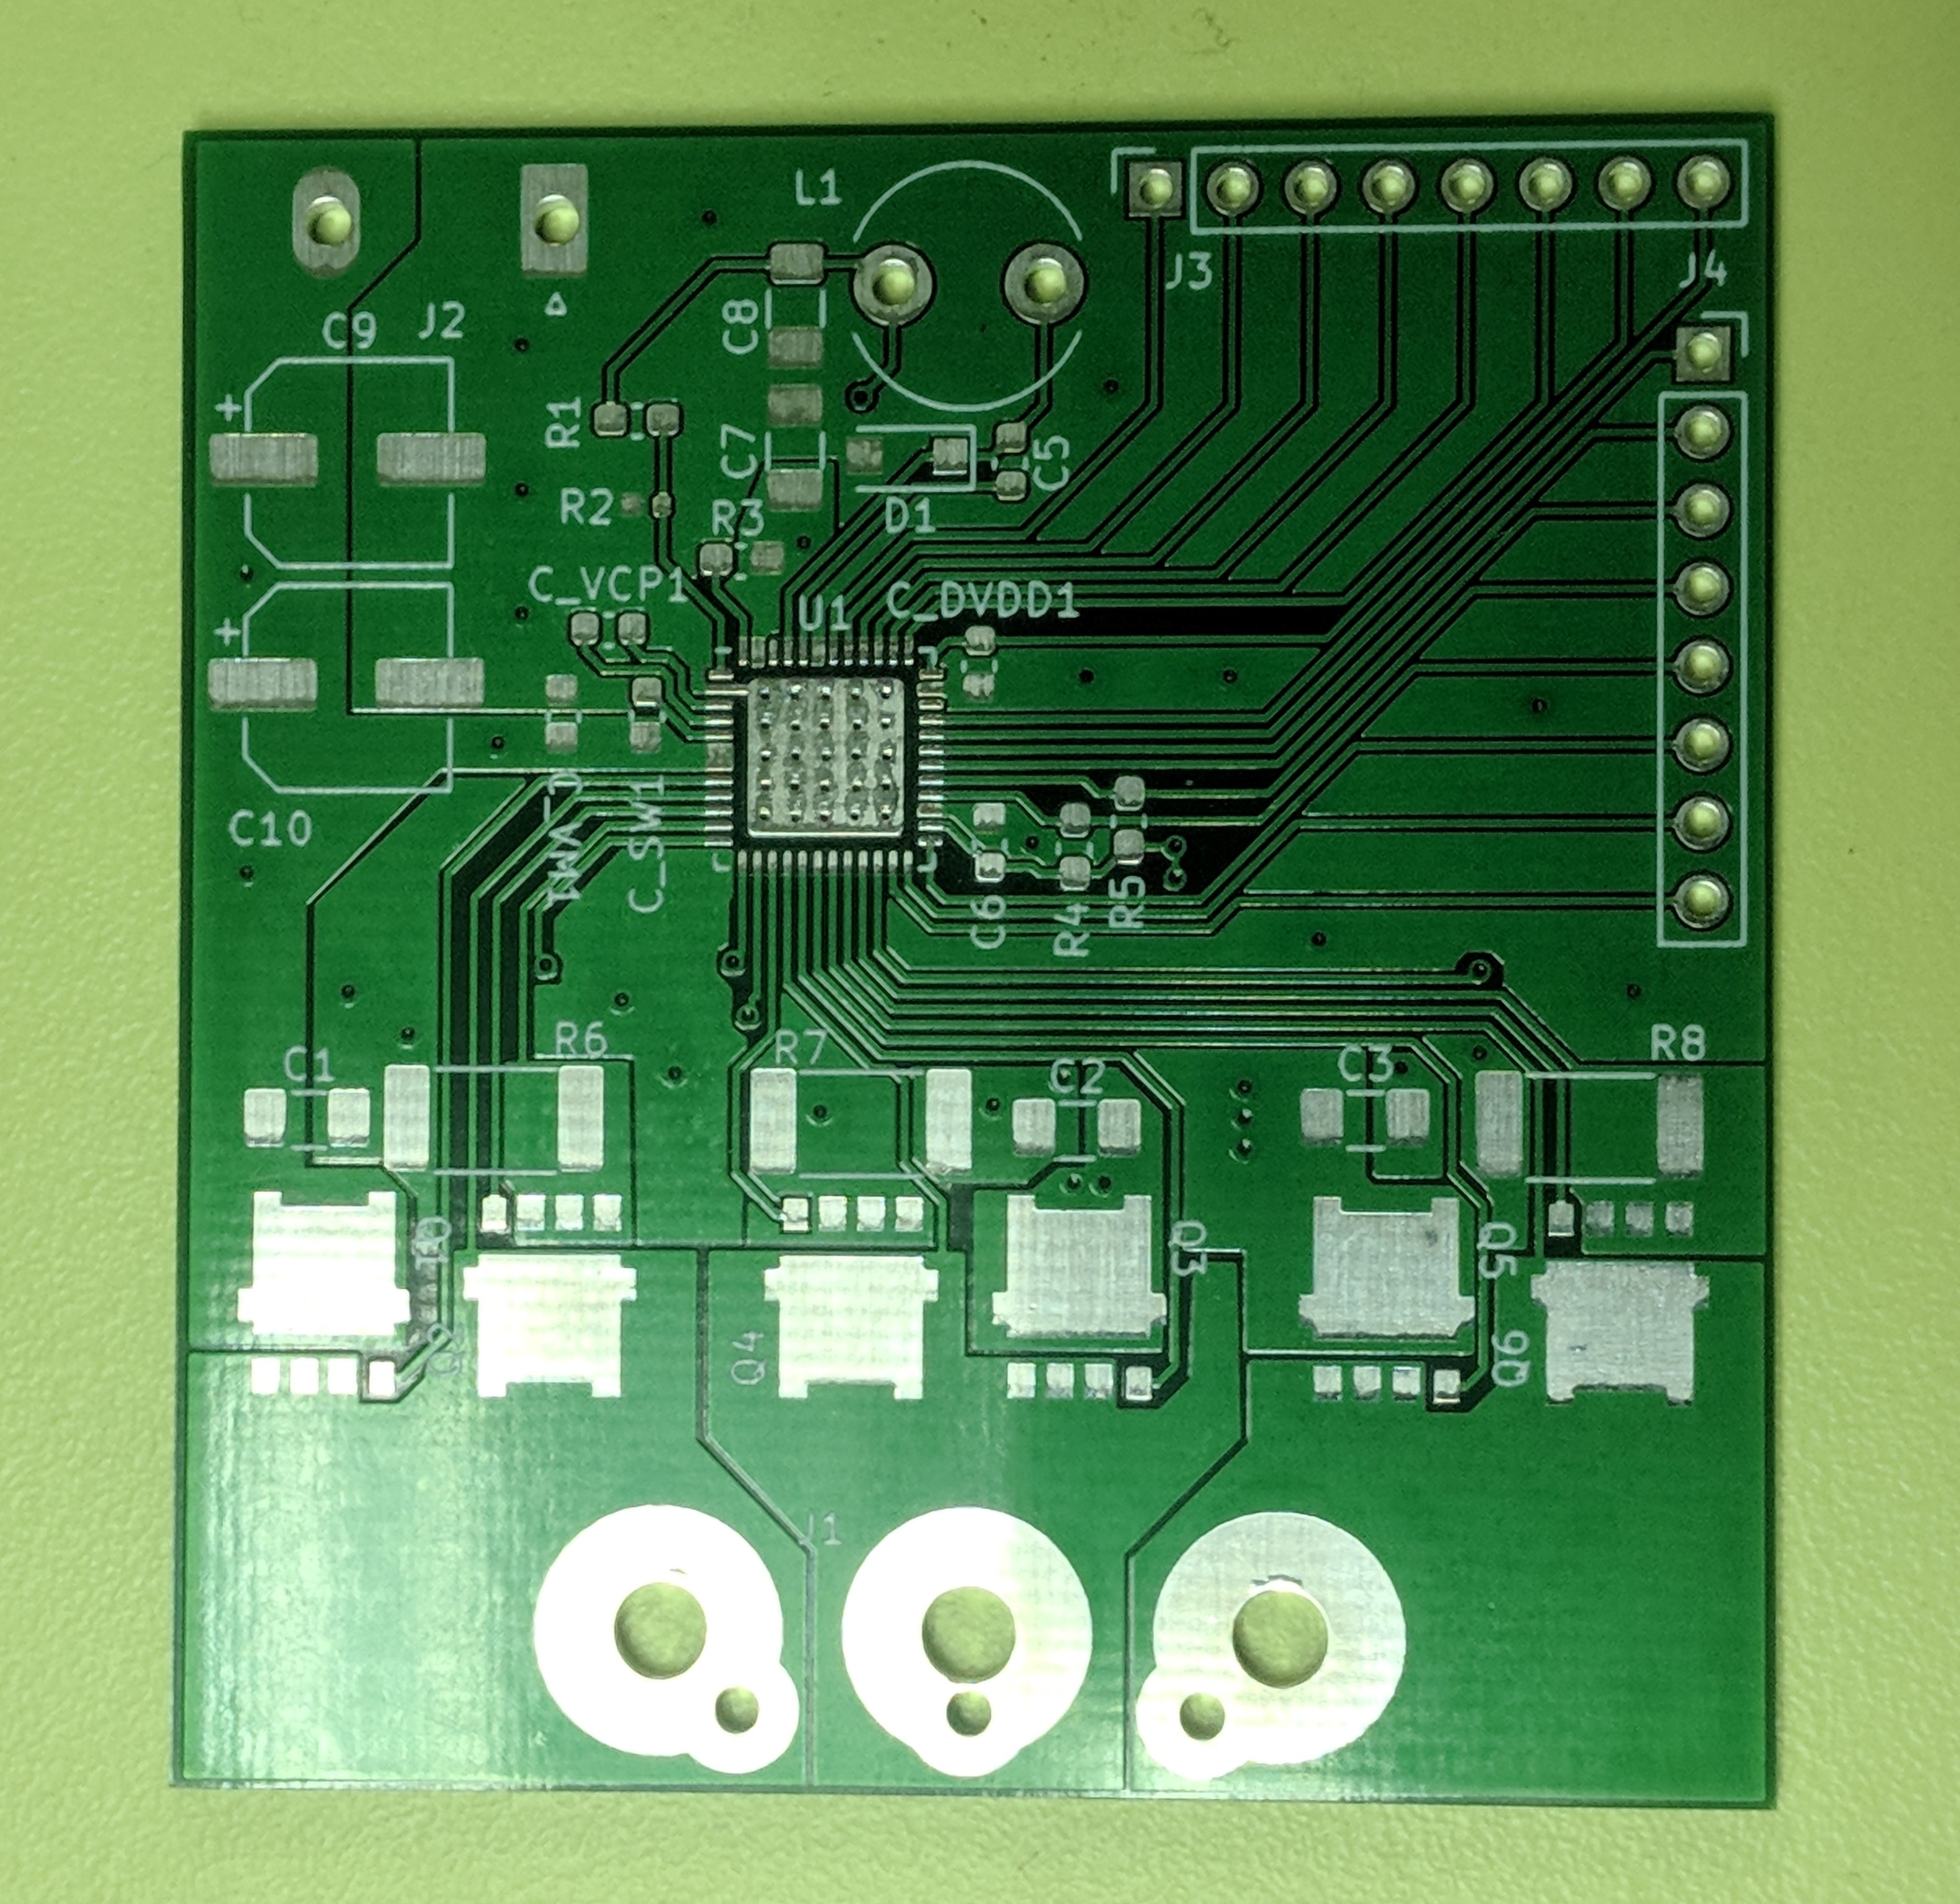
\includegraphics[width=0.4\columnwidth]{images/joint_controller_pcb_top}
\par\end{centering}
}
\par\end{centering}
\begin{centering}
\subfloat[Bottom Layer]{\begin{centering}
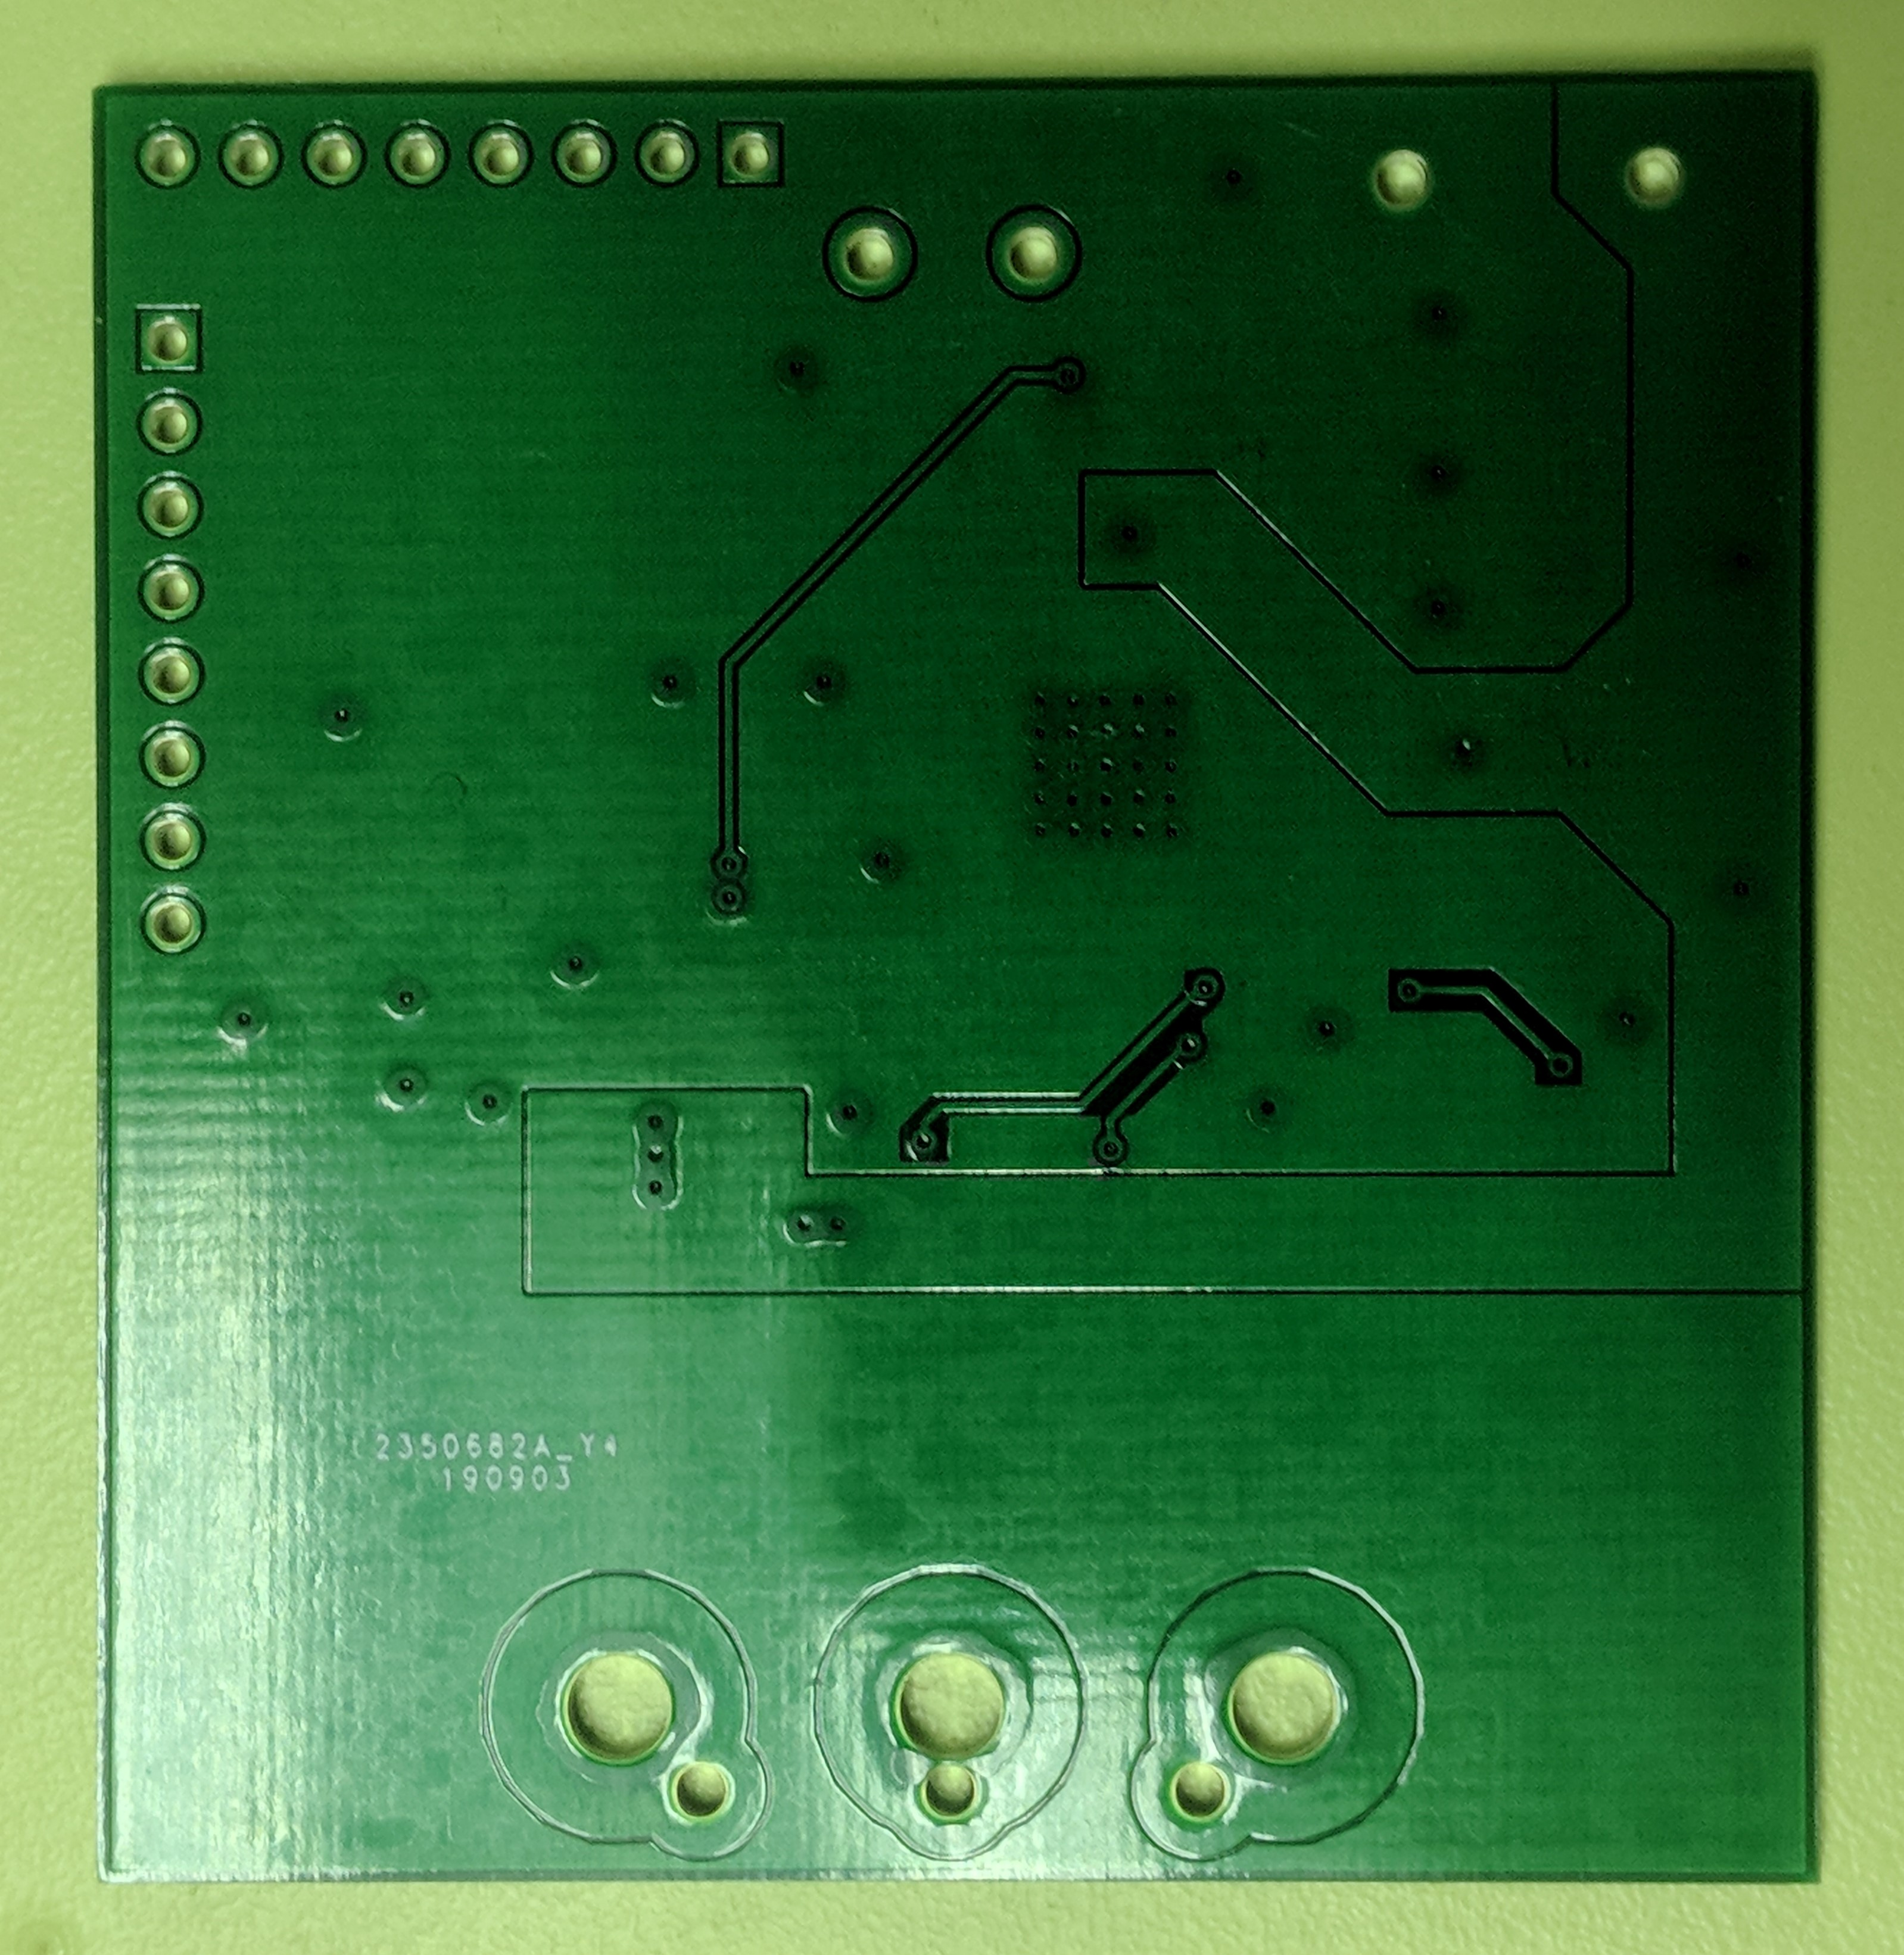
\includegraphics[width=0.4\columnwidth]{images/joint_controller_pcb_bottom}
\par\end{centering}
}
\par\end{centering}
\caption{Unpopulated Joint Controller PCB\label{fig:joint-controller-pcb}}
\end{figure}

\begin{figure}[H]
\begin{centering}
\subfloat[Top Layer]{\begin{centering}
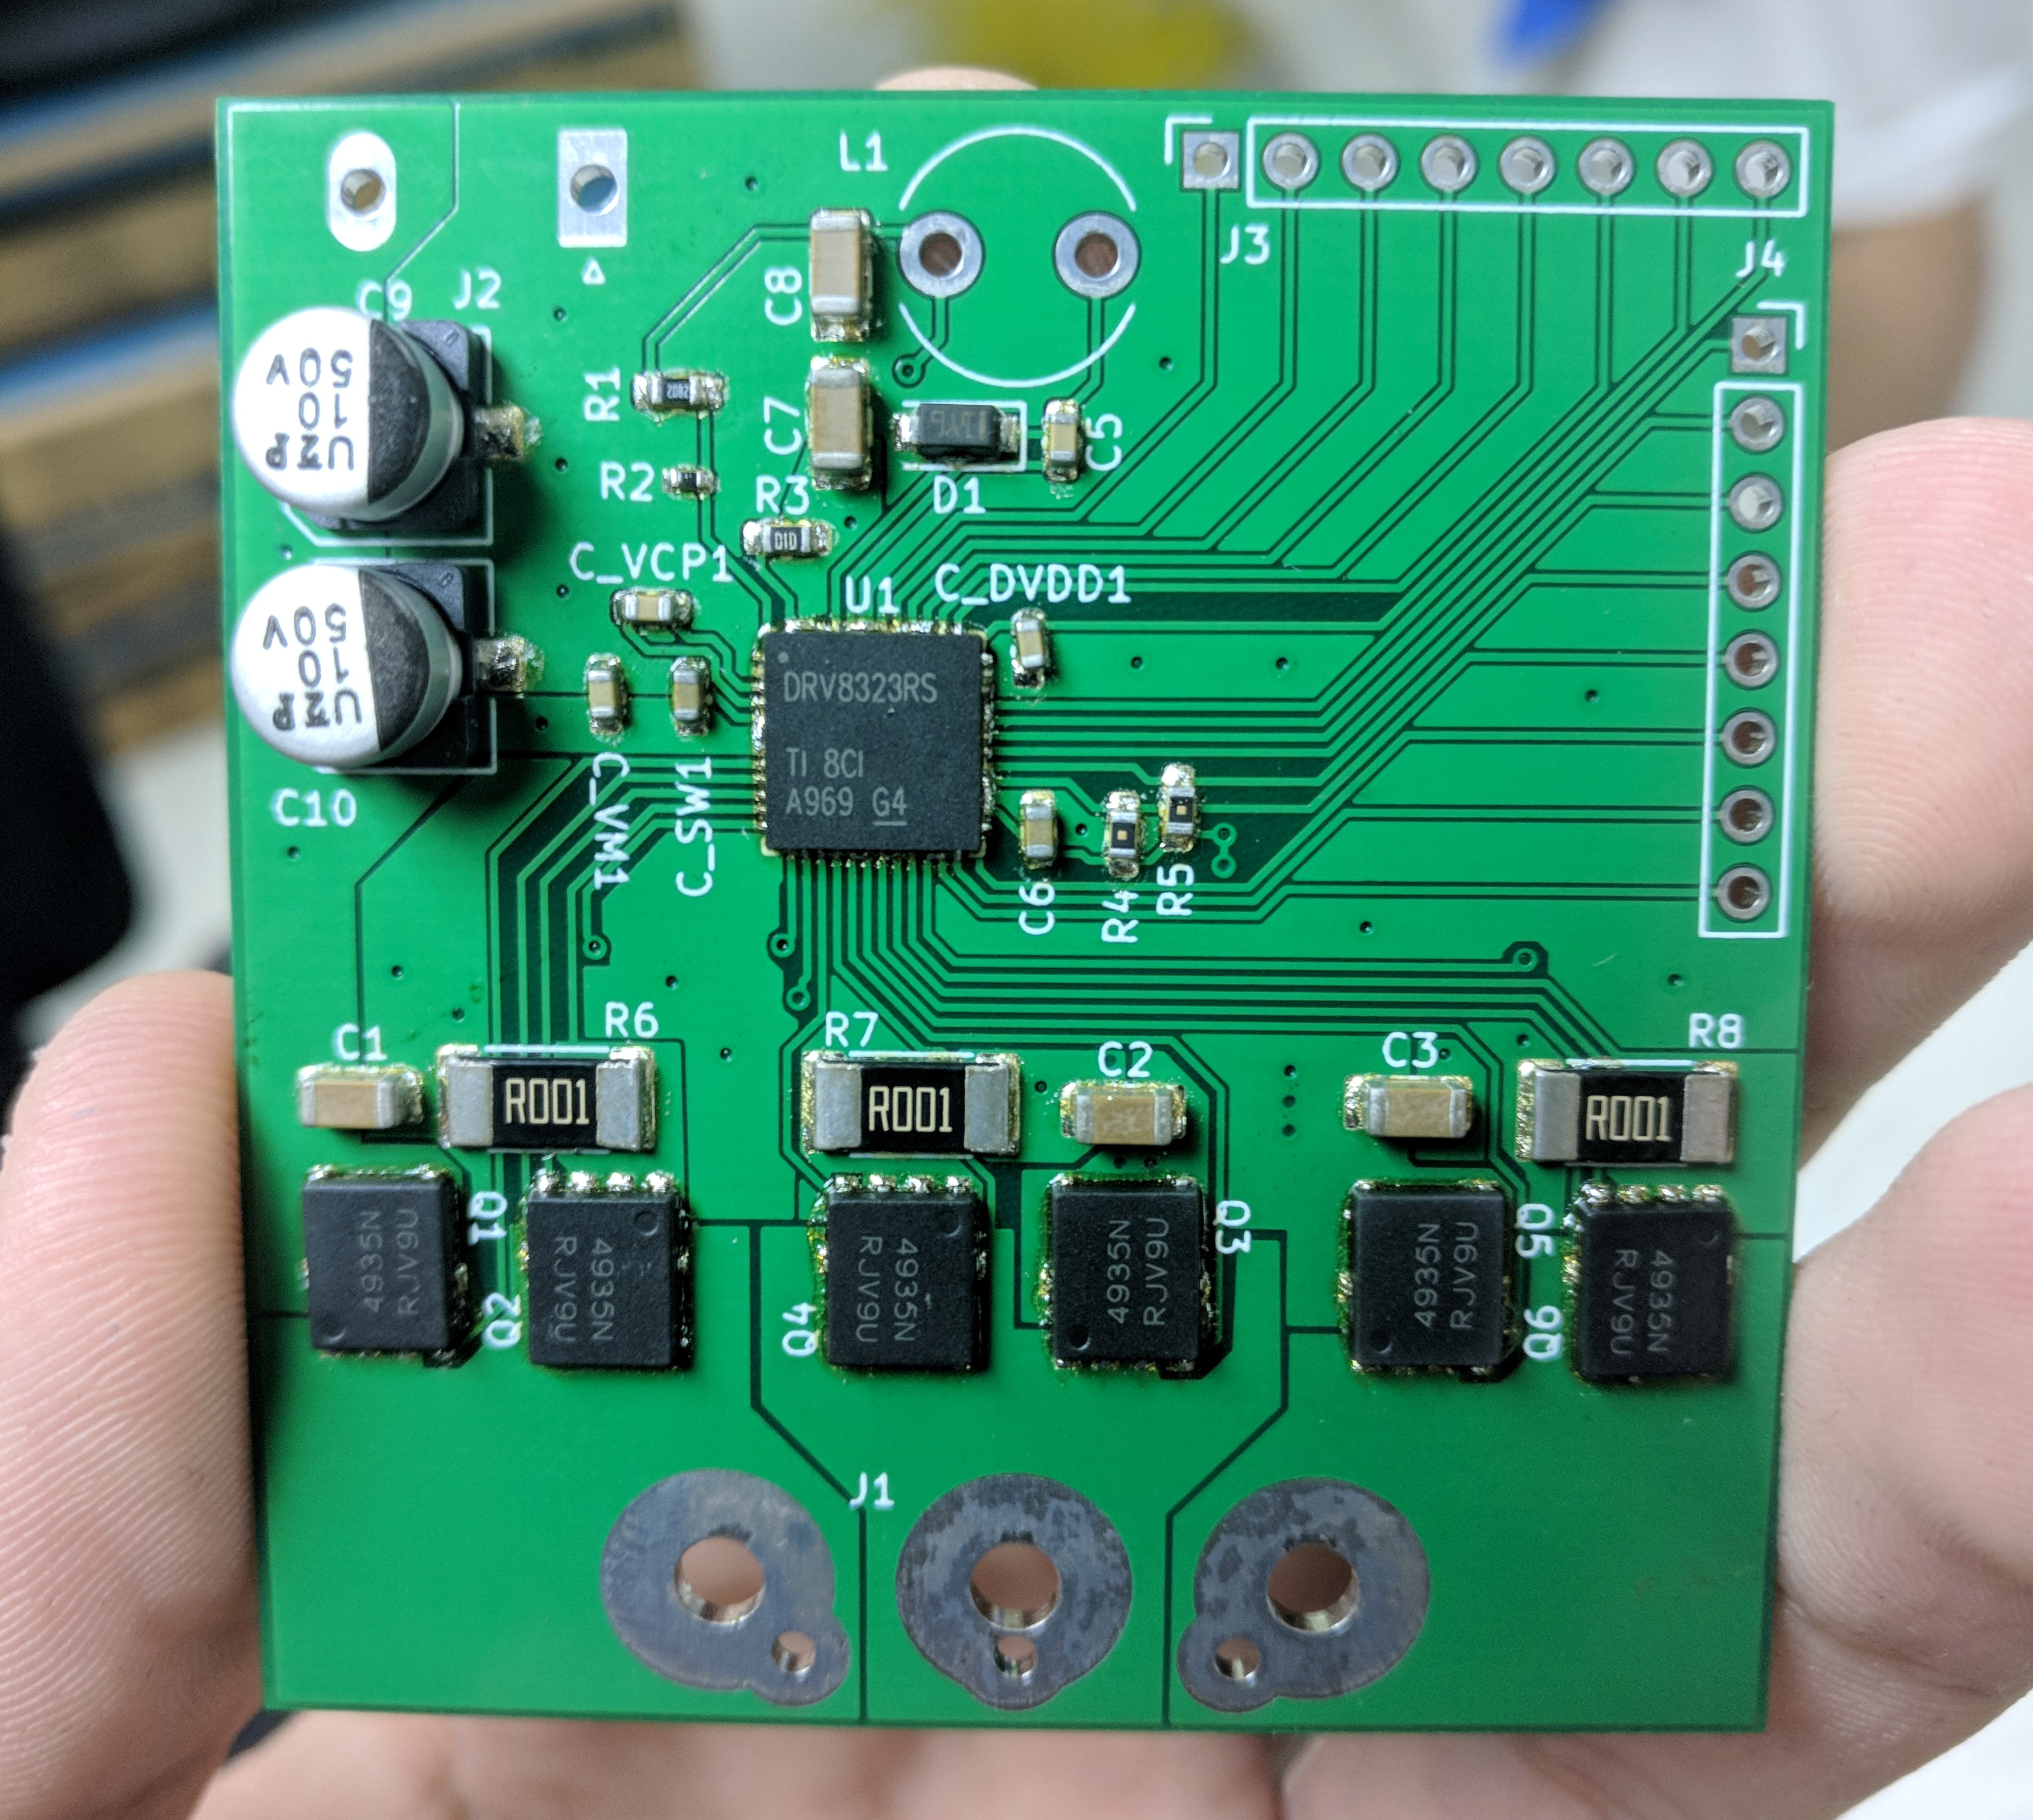
\includegraphics[width=0.4\columnwidth]{images/joint_controller_pcb_top_full}
\par\end{centering}
}
\par\end{centering}
\begin{centering}
\subfloat[Bottom Layer]{\begin{centering}
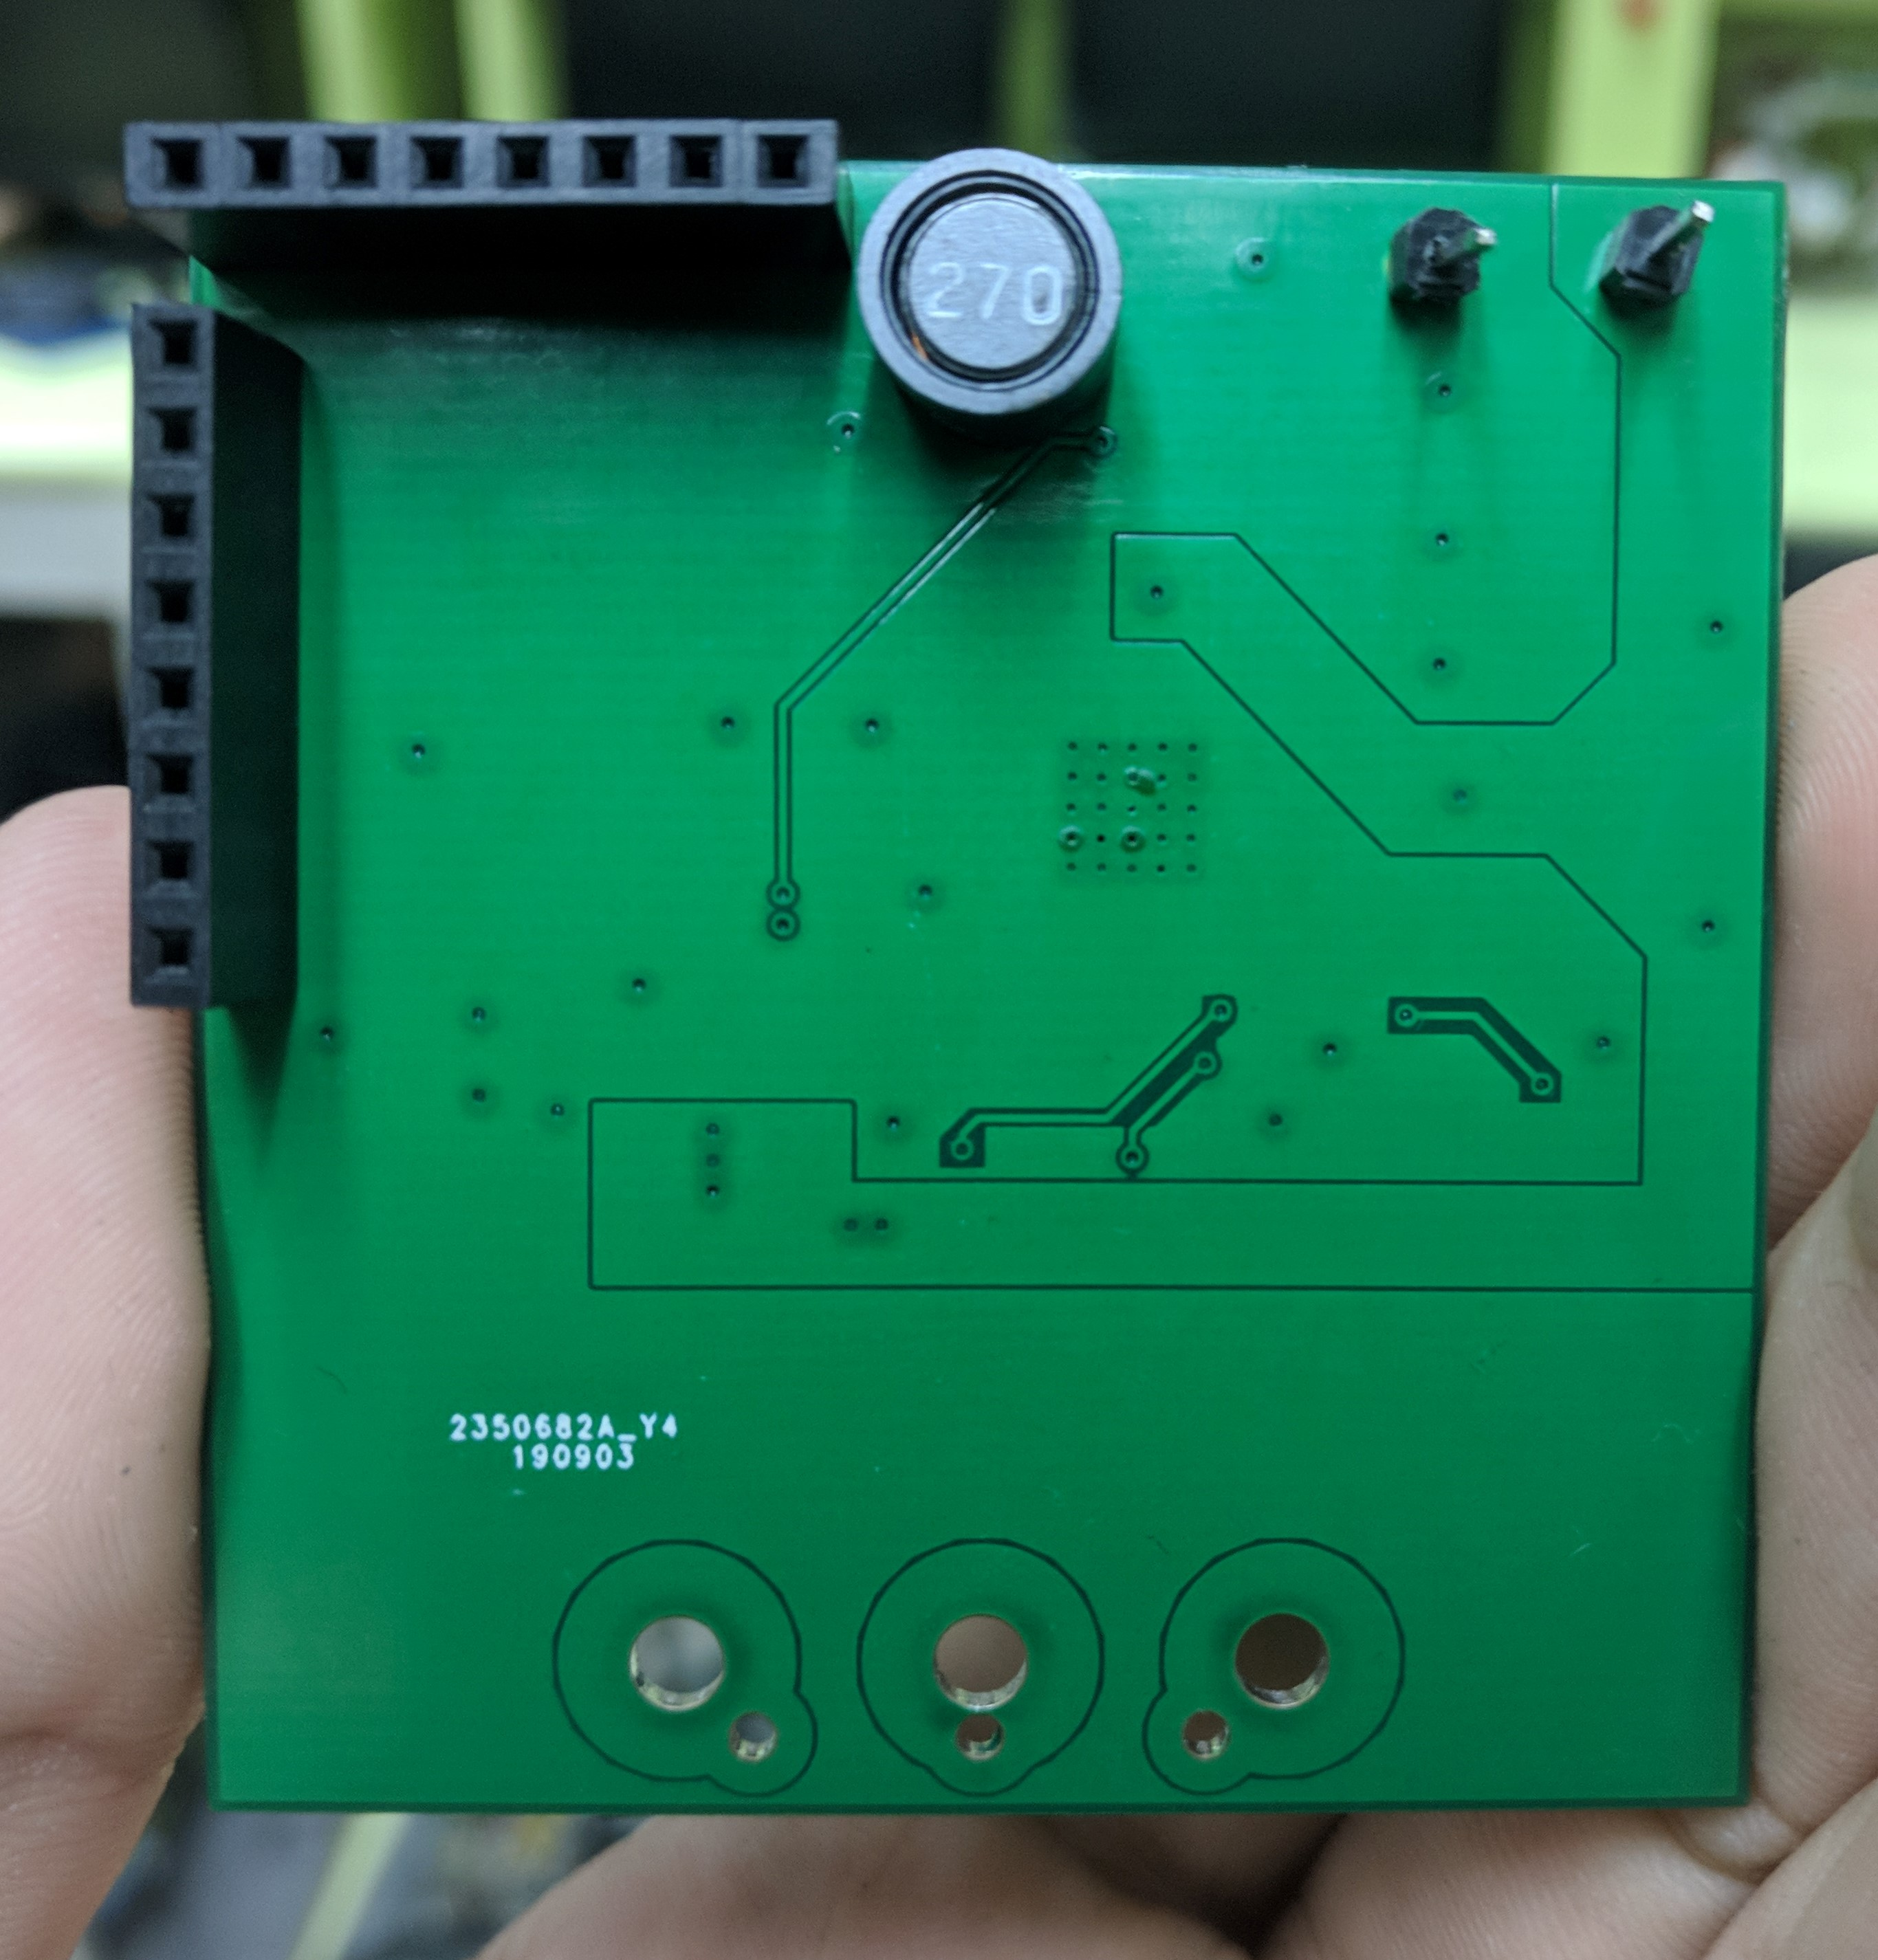
\includegraphics[width=0.4\columnwidth]{images/joint_controller_pcb_bottom_full}
\par\end{centering}
}
\par\end{centering}
\caption{Populated Joint Controller PCB\label{fig:joint-controller-pcb-full}}
\end{figure}

\section{Control}

Field-Oriented Control is implemented on a dsPIC33CK256MP508 Curiosity Development Board aside from the PLL Estimator Block. The low-pass filtered output of the SVM block is shown in Figure \ref{fig:svm-output}.

\begin{figure}[H]
\begin{centering}
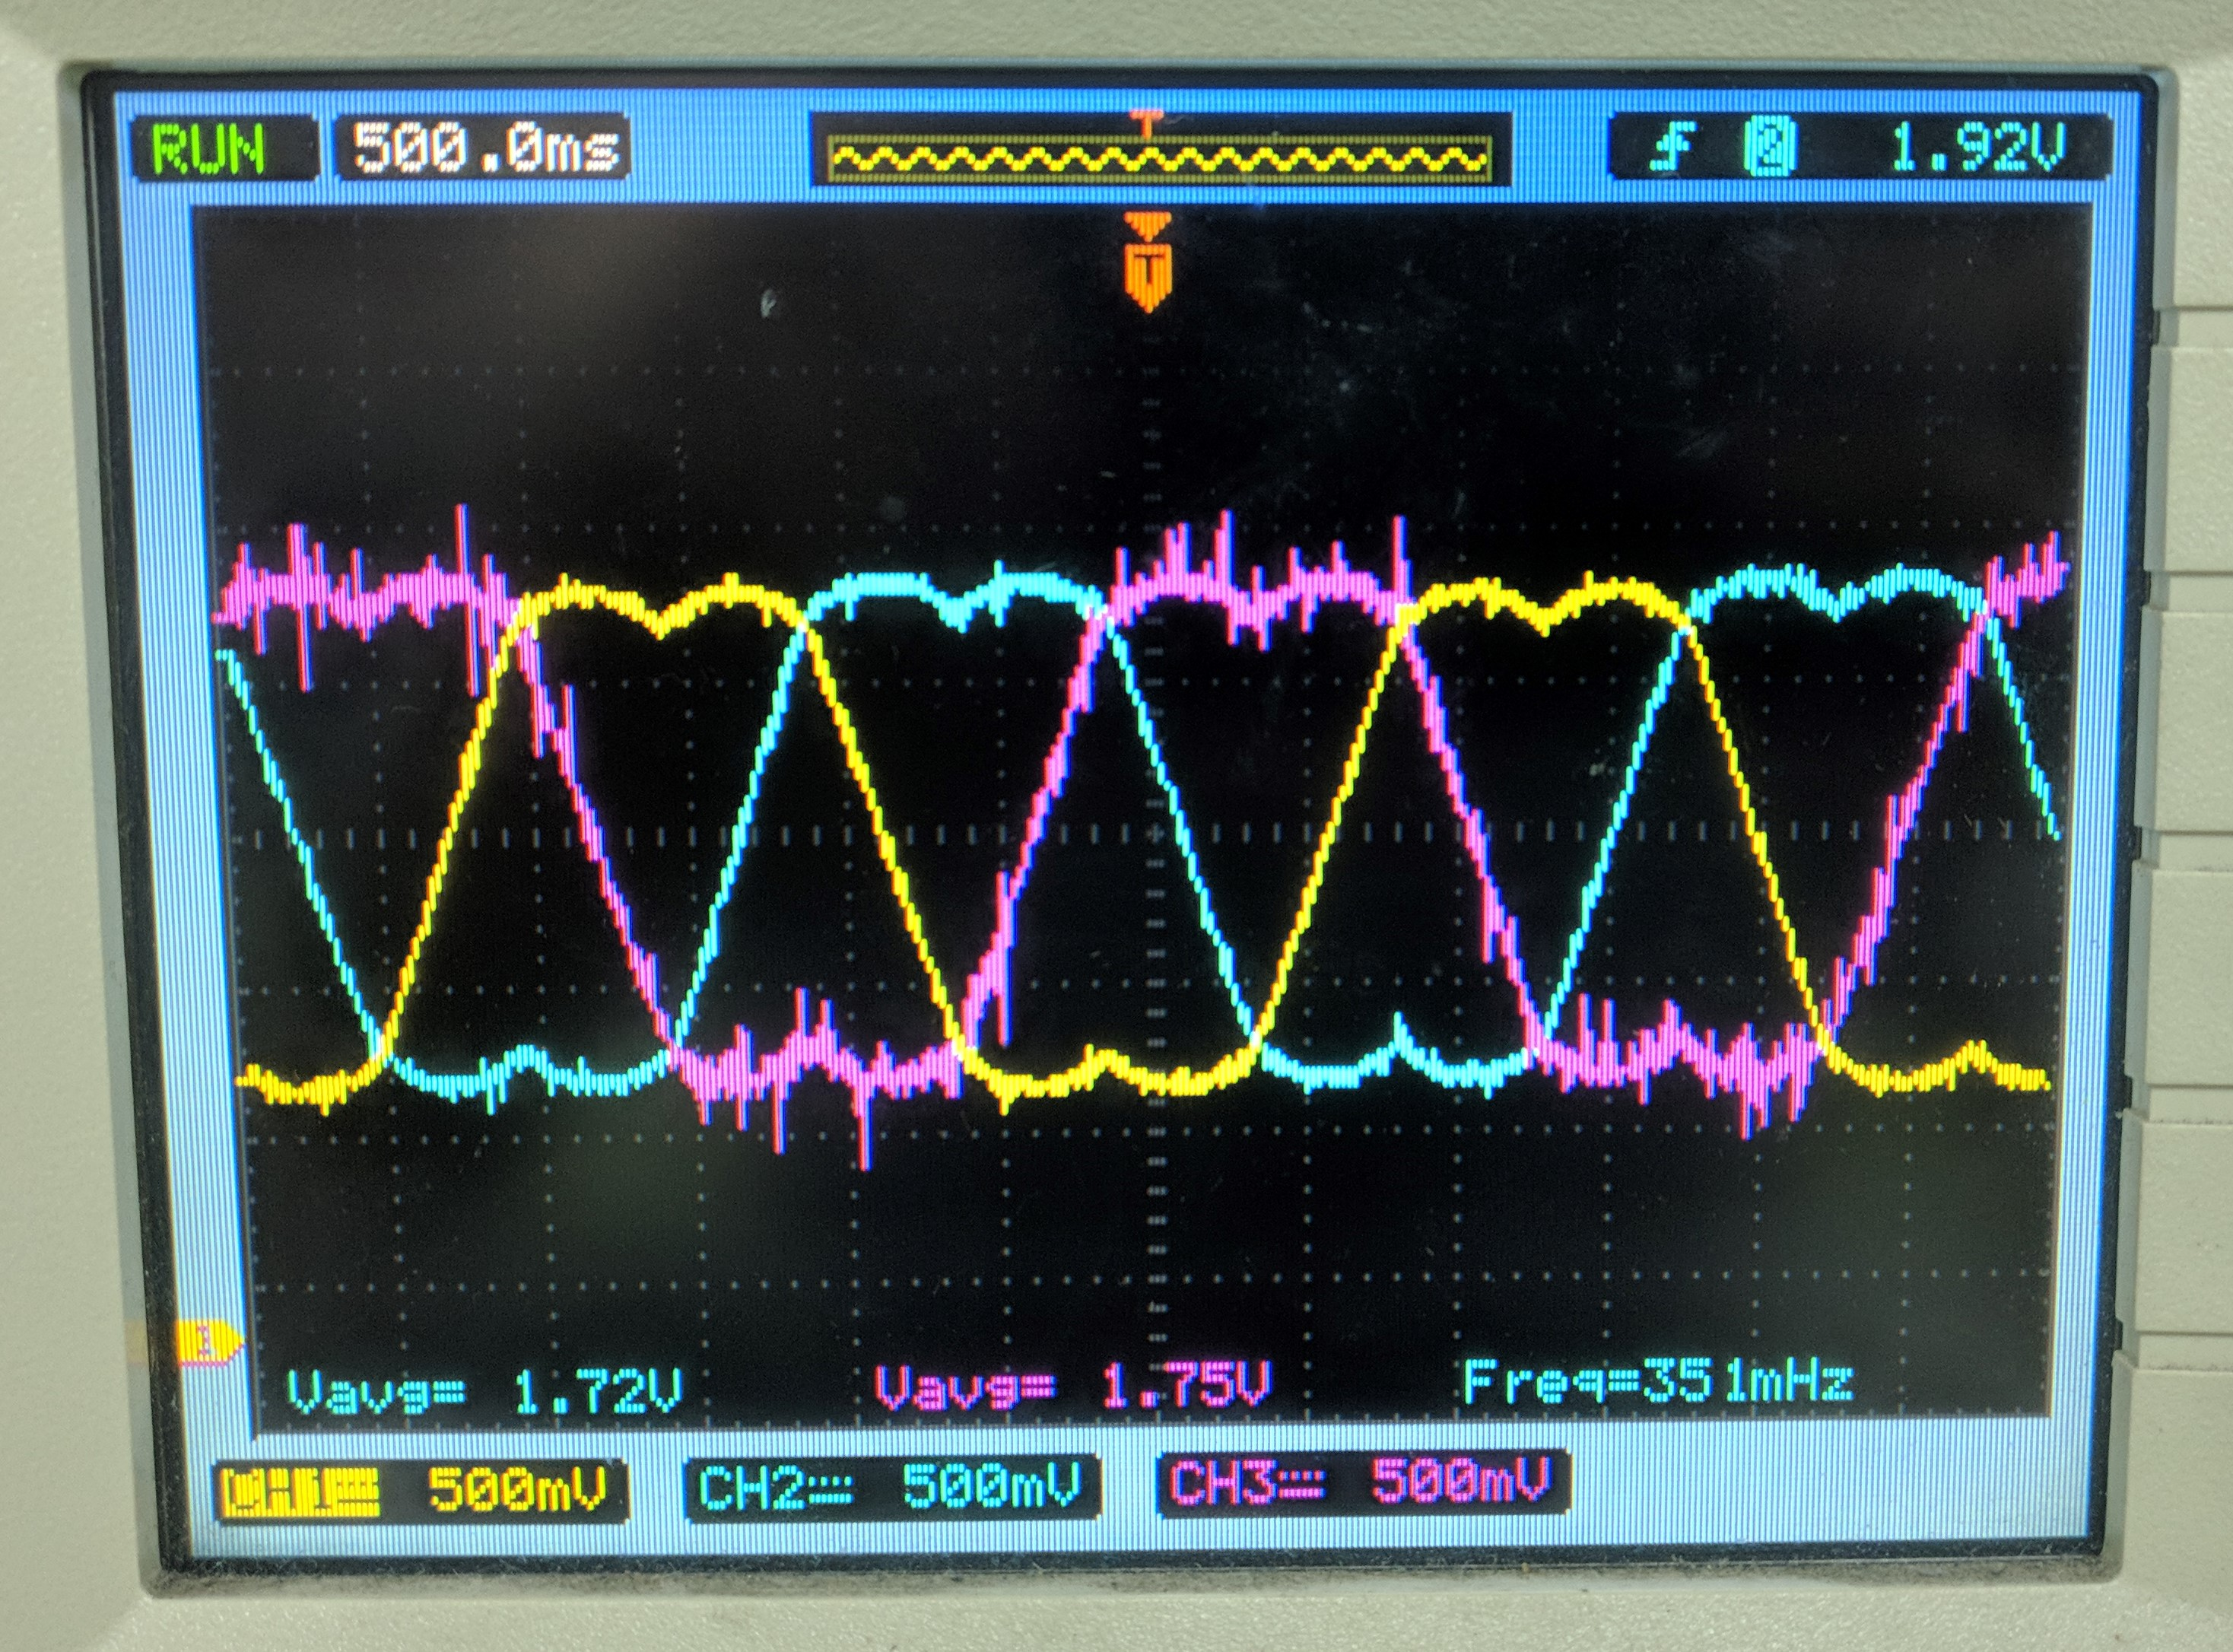
\includegraphics[width=0.7\columnwidth]{images/svm}
\par\end{centering}
\caption{Space Vector Modulation Low-Pass Output\label{fig:svm-output}}
\end{figure}

\cleardoublepage{}

\chapter{Project Schedule and Deliverables\label{cha:Project-Sked}}

The project is to be done during the 2nd Semester of Academic Year 2019-2020 for 17 weeks starting on January 10, 2020. The halfway point of the project will be evaluated 8 weeks after starting. The overall timeline for the project is shown as a gantt chart in Figure \ref{fig:gantt-chart}. Each period interval is one week long.

\section{Gantt Chart }

\begin{figure}[H]
\begin{centering}
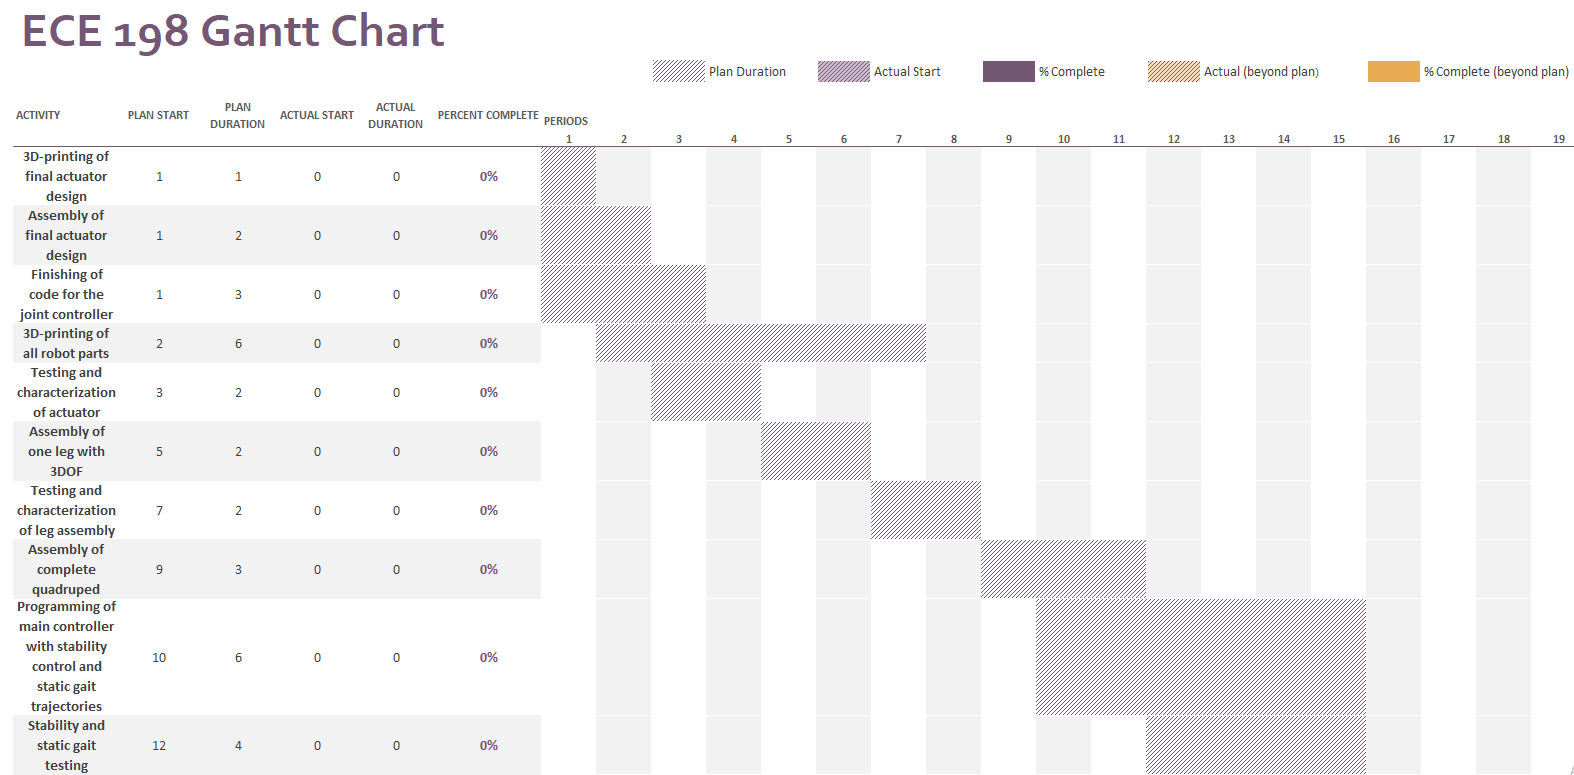
\includegraphics[width=1.0\columnwidth]{images/gantt_chart}
\par\end{centering}
\caption{EEE 198 Gantt Chart\label{fig:gantt-chart}}
\end{figure}

\section{Halfway-point Deliverables}

This section should clearly point out and describe the expected outputs
at halfway-point. If the project will be done by a group, the deliverables
of each group member shall be clearly and specifically stated. 

\section{Final Deliverables}

This section should clearly point out the final deliverables. If the
project will be done by a group, the deliverables of each group member
shall be clearly and specifically stated.

\cleardoublepage{}

\bibliographystyle{unsrt}
\nocite{*}
\bibliography{bibliography}

\cleardoublepage{}

\appendix

\chapter{PopBit Technical Datasheets}

\begin{figure}[H]
\begin{centering}
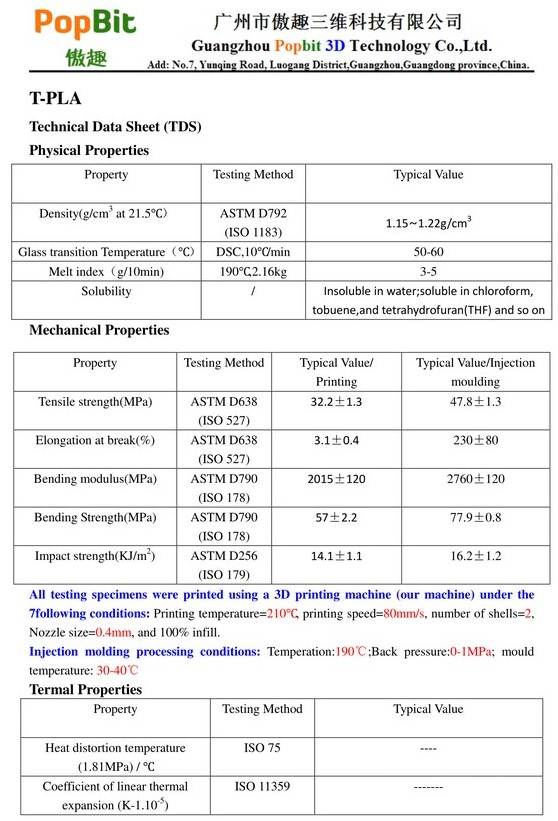
\includegraphics[width=0.8\columnwidth]{images/tpla}
\par\end{centering}
\caption{T-PLA Technical Datasheet\label{fig:tpla}}
\end{figure}

\begin{figure}[H]
\begin{centering}
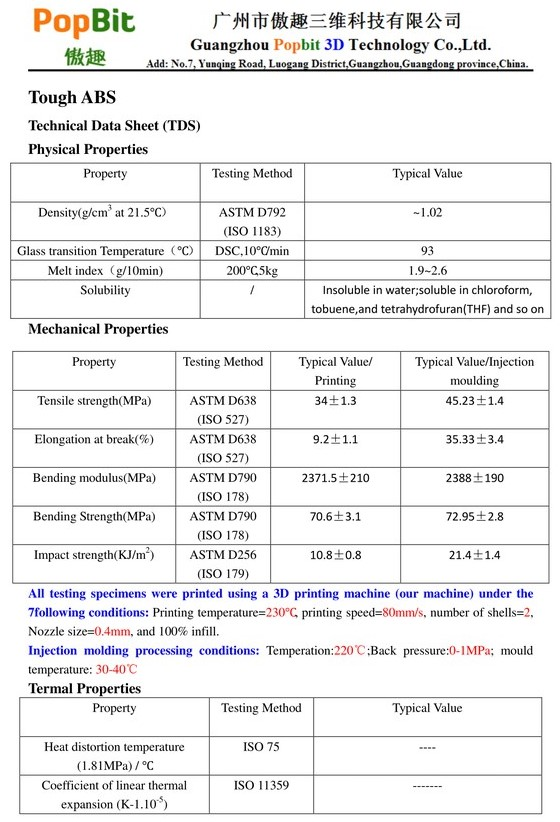
\includegraphics[width=0.8\columnwidth]{images/tabs}
\par\end{centering}
\caption{T-ABS Technical Datasheet\label{fig:tabs}}
\end{figure}

\cleardoublepage
\end{document}
